% ==============================================================================
% 02_differences_milieu.tex - Module 2 (10h30 - 12h00)
% Présentation d'un drone sous-marin : différences avec le drone aérien
% Fabrication réelle : Enceintes 3"/4", Pénétrateurs WetLink, Connecteurs Cobalt & SubConn, Test de vide, BlueBoat, DVL-A50
% ==============================================================================

\section{Module 2 : Différences avec l'Aérien \& Spécificités du Milieu}

\begin{frame}{2.1 Deux Mondes Physiques Opposés}
  \begin{table}[h]
    \centering
    \small
    \begin{tabularx}{\textwidth}{l X X}
      \toprule
      \textbf{Caractéristique} & \textbf{Milieu Aérien (UAV)} & \textbf{Milieu Marin (AUV / ROV)} \\
      \midrule
      \textbf{Masse volumique $\rho$} & $\approx 1.2\,\text{kg/m}^3$ & $\approx 1025\,\text{kg/m}^3$ \alertw{($\times 850$)} \\
      \textbf{Génération de force} & Portance aérodynamique ($v^2$) & Poussée d'Archimède statique \\
      \textbf{Stabilité naturelle} & Instable actif (quadrotor) & \succw{Stabilité statique passive ($B$ sur $G$)} \\
      \textbf{Pression ambiante} & $\approx 1\,\text{bar}$ (décroît) & $+1\,\text{bar}$ tous les $10\,\text{m}$ \\
      \textbf{Ondes radio / GNSS} & Propagation libre (GPS, 4G, WiFi) & \alertw{Absorption totale en qqs cm} \\
      \textbf{Visibilité / Optique} & Kilométrique & Métrique ($1\text{--}15\,\text{m}$), turbidité \\
      \textbf{Agression chimique} & Faible & Corrosion saline, conductivité \\
      \bottomrule
    \end{tabularx}
  \end{table}
\end{frame}

\begin{frame}{2.2 Hydrostatique : Flottabilité et Stabilité Passive}
  \begin{columns}[c]
    \begin{column}{0.44\textwidth}
      \begin{center}
        \begin{tikzpicture}[scale=0.82]
          % Corps de drone sous-marin
          \draw[thick, fill=OceanMedium!10, rounded corners=10pt] (-1.5,-1.3) rectangle (1.5,1.3);
          
          % Centre de carène B (haut)
          \coordinate (B) at (0, 0.65);
          \fill[OceanCyan] (B) circle (3.5pt);
          \draw[->, line width=1.8pt, OceanCyan] (B) -- (0, 1.85) node[above] {\small Poussée d'Archimède $\vec{F}_B$};
          \node[right=3pt of B] {\footnotesize \textbf{Centre de Carène $B$}};

          % Centre de gravité G (bas)
          \coordinate (G) at (0, -0.65);
          \fill[OceanDeep] (G) circle (3.5pt);
          \draw[->, line width=1.8pt, OceanCoral] (G) -- (0, -1.85) node[below] {\small Poids $\vec{P} = m\vec{g}$};
          \node[right=3pt of G] {\footnotesize \textbf{Centre de Gravité $G$}};

          % Bras de levier BG
          \draw[<->, thick, dashed] (-0.3,-0.6) -- (-0.3,0.6) node[midway, left] {\small $\overline{BG} > 0$};
        \end{tikzpicture}
      \end{center}
    \end{column}

    \begin{column}{0.54\textwidth}
      \small
      \textbf{Règle d'or de l'ingénierie sous-marine} :
      \begin{itemize}\setlength{\itemsep}{2pt}\setlength{\parskip}{0pt}
        \item Masses lourdes (batteries, caisson bas) \textbf{en bas}.
        \item Mousses flottantes (PEHD / syntactique) \textbf{en haut}.
        \item Couple de rappel hydrostatique :
        \begin{equation*}
          \setlength{\abovedisplayskip}{2pt}
          \setlength{\belowdisplayskip}{2pt}
          C_{\text{rappel}} = m \cdot g \cdot \overline{BG} \cdot \sin(\theta)
        \end{equation*}
        \item Drone \tech{auto-redressant} en roulis ($\phi$) et tangage ($\theta$) : zéro énergie dépensée pour rester horizontal !
      \end{itemize}

      \vspace{0.2em}
      \begin{block}{Flottabilité Positive de Sécurité}
        Lestage réglé pour $+200$ à $+500\,\text{g}$ nets : en cas de coupure de batterie, le robot \succw{remonte seul en surface}.
      \end{block}
    \end{column}
  \end{columns}
\end{frame}

\begin{frame}{2.3 Conception Réelle des Caissons Étanches (Modulaire 2" à 8")}
  \begin{columns}[c]
    \begin{column}{0.56\textwidth}
      \begin{block}{\tech{Gamme de Diamètres (2" à 8") \& Matériaux}}
        \scriptsize
        \begin{itemize}
          \item \textbf{Diamètres modulaires} : du \textbf{2"} (capteurs/éclairages), \textbf{3"} (batteries) et \textbf{4"} (électronique) jusqu'au \textbf{6"} et \textbf{8"} (gros payloads / AUV / baies de puissance).
          \item \textbf{Acrylique (PMMA)} : transparent, vue caméra \& voyants ($100\text{--}150\,\text{m}$).
          \item \textbf{Alu 6061-T6 anodisé dur} : certifié \succw{$\mathbf{400\text{--}500\,\text{m}}$}, dissipation thermique active des ESC / processeurs.
        \end{itemize}
      \end{block}

      \begin{block}{\succw{Flasques, Bouchons \& Verrouillage}}
        \scriptsize
        \begin{itemize}
          \item \textbf{Types d'embouts} : dômes optiques hémisphériques (caméras), flasques plates alu/acrylique (aveugles ou pré-percées 4 à 18 trous M10/M14).
          \item \textbf{Systèmes de fermetures} : cordon de verrouillage (*Locking Cord*) sans vis traversantes ou brides boulonnées.
          \item \textbf{Étanchéité} : double joint torique (*O-ring* radial + facial).
        \end{itemize}
      \end{block}
    \end{column}

    \begin{column}{0.42\textwidth}
      \begin{center}
        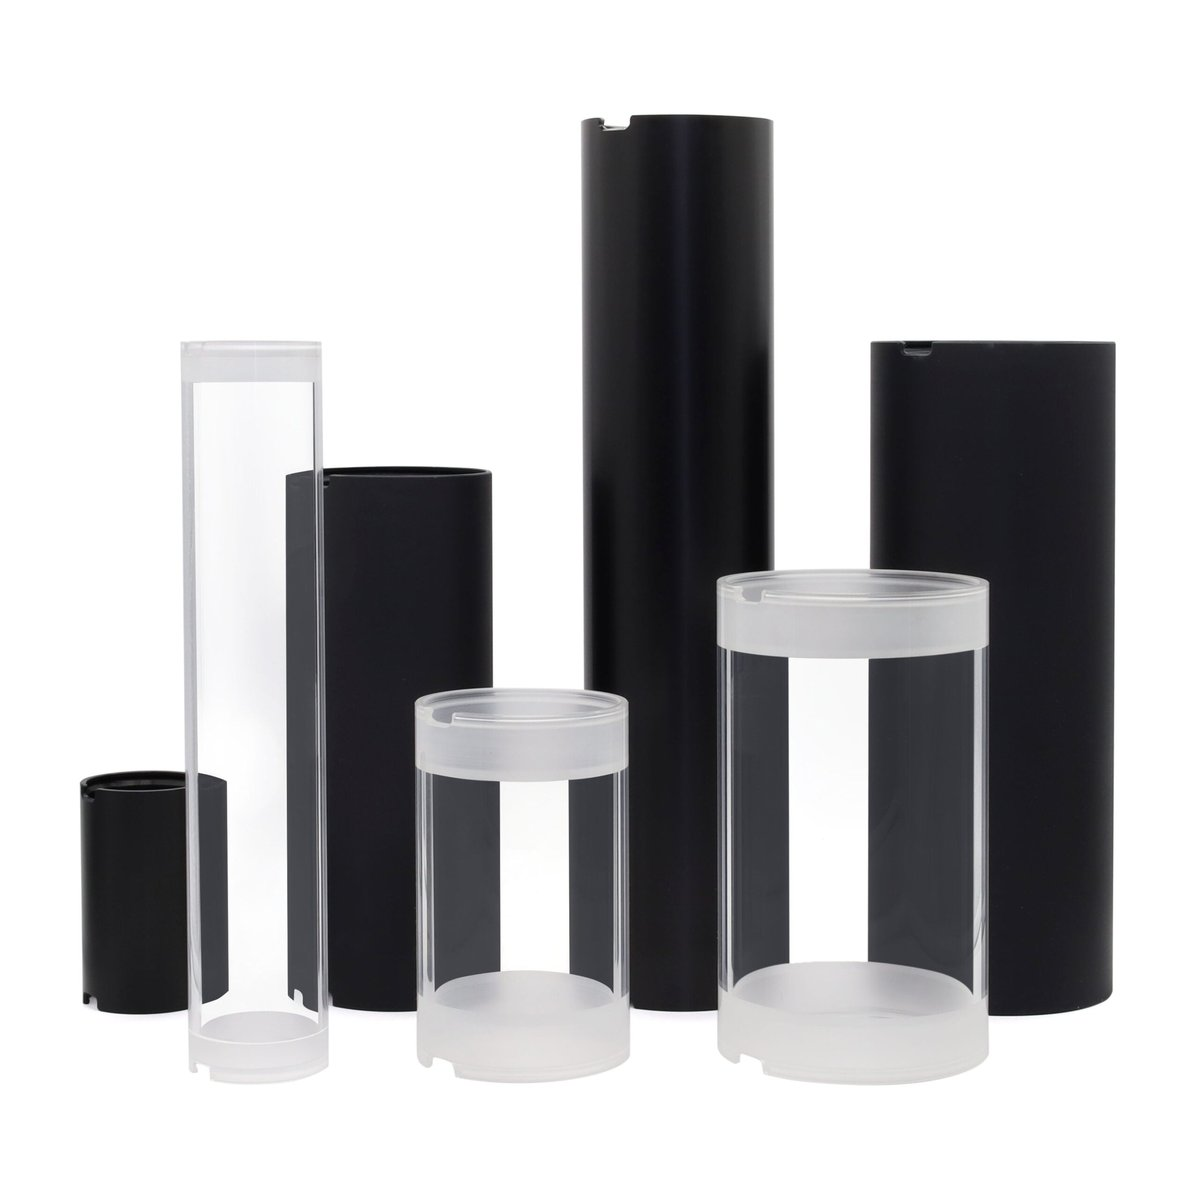
\includegraphics[width=\textwidth, height=3.6cm, keepaspectratio]{watertight_enclosure.jpg}\\
        \vspace{0.2em}
        \footnotesize\textbf{Caisson Étanche Modulaire (ex. 4")}\\
        \scriptsize\textit{Tube alu/acrylique, flasques O-ring, locking cord \& dôme optique}
      \end{center}
    \end{column}
  \end{columns}
\end{frame}

\begin{frame}{2.4 Franchissement de Paroi : WetLink Standard vs Nouveau JPT}
  \begin{block}{\succw{Révolution WetLink : La Fin Définitive du Potting Époxy}}
    \scriptsize
    L'ancienne coulée de résine époxy prenait 24h et était irréversible. Les pénétrateurs brevetés WetLink s'assemblent en \succw{\textbf{30 secondes}}, sans colle, et restent \succw{\textbf{100\% réutilisables}} en maintenance.
  \end{block}

  \vspace{-0.3em}
  \begin{columns}[T]
    \begin{column}{0.48\textwidth}
      \begin{center}
        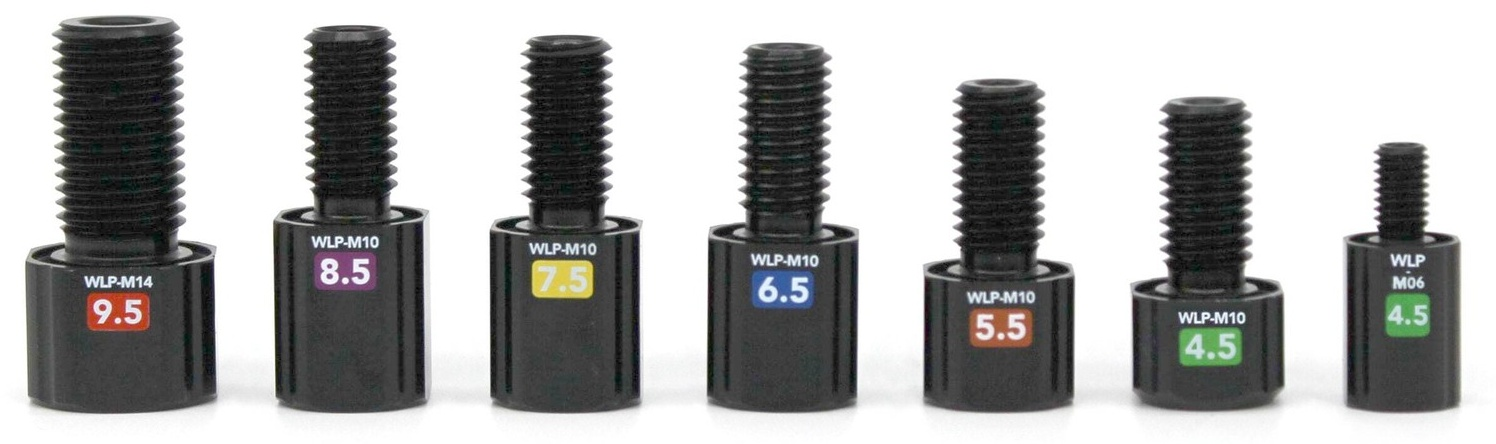
\includegraphics[height=1.75cm, width=\textwidth, keepaspectratio]{wetlink_penetrator_clean.jpg}\\
        \vspace{0.15em}
        \tech{1. WetLink Penetrator Standard (WLP)}\\
        \tiny\textit{Compression sur isolants individuels $\cdot$ Haute pression \textbf{950 m}}
      \end{center}
      \scriptsize
      \begin{itemize}\setlength{\itemsep}{1.5pt}\setlength{\parskip}{0pt}
        \item \textbf{Principe} : compression conique du joint \alertw{sur les conducteurs internes}.
        \item \textbf{Préparation} : nécessite de \alertw{dénuder la gaine extérieure} ($\approx 15\,\text{mm}$).
        \item \textbf{Usage cible} : thrusters T200, ombilic Fathom, traversées haute pression.
      \end{itemize}
    \end{column}

    \begin{column}{0.48\textwidth}
      \begin{center}
        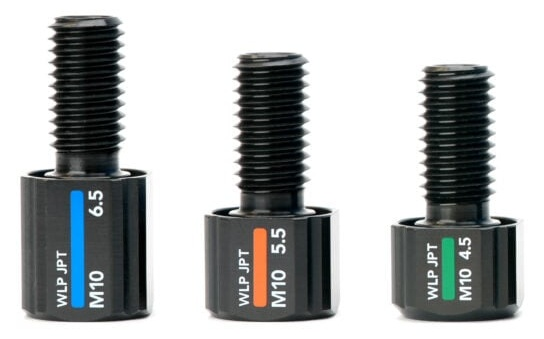
\includegraphics[height=1.75cm, width=\textwidth, keepaspectratio]{wetlink_jpt_clean.jpg}\\
        \vspace{0.15em}
        \succw{2. Nouveau WetLink JPT (Jacket Pass-Through)}\\
        \tiny\textit{Traversée intégrale directe avec gaine $\cdot$ Pression max \textbf{100 m}}
      \end{center}
      \scriptsize
      \begin{itemize}\setlength{\itemsep}{1.5pt}\setlength{\parskip}{0pt}
        \item \textbf{Principe} : \succw{zéro dénudage}, le câble complet traverse avec sa gaine.
        \item \textbf{Étanchéité} : joint conique serrant la gaine ($4.5$, $5.5$ ou $6.5\,\text{mm}$).
        \item \textbf{Usage cible} : coaxiaux d'antenne, blindés vidéo ou capteurs modulaires.
      \end{itemize}
    \end{column}
  \end{columns}
\end{frame}

\begin{frame}{2.5 Pénétrateurs vs Connecteurs : Maintenance \& Modularité}
  \begin{columns}[T]
    \begin{column}{0.49\textwidth}
      \begin{block}{\alertw{Cas Concret : Moteur Défaillant en Manip}}
        \scriptsize
        \begin{itemize}
          \item \textbf{Avec Pénétrateur Fixe (WetLink / Époxy)} :
            \begin{enumerate}\tiny
              \item Rinçage \& séchage intégral extérieur.
              \item Ouvrir le caisson, extraire le tiroir électronique.
              \item Dessouder/dévisser les 3 phases moteur.
              \item Dévisser le contre-écrou interne M10.
              \item Câbler le rechange, refermer, \alertw{refaire 15 min de vide}.
            \end{enumerate}
            $\rightarrow$ \textbf{1h30 d'arrêt}, impossible sur semi-rigide !
          \item \textbf{Avec Connecteur Étanchéifié Externe} :
            \begin{itemize}\tiny
              \item Dévisser la bague, débrancher le moteur en panne.
              \item Brancher le moteur de rechange, revisser la bague.
              \item \succw{2 minutes chrono sans ouvrir le caisson !}
              \item Vide intact, zéro risque d'embruns salés.
            \end{itemize}
        \end{itemize}
      \end{block}
    \end{column}

    \begin{column}{0.49\textwidth}
      \begin{block}{\succw{Modularité "À la Volée" des Capteurs}}
        \scriptsize
        \begin{itemize}
          \item \textbf{Ports Auxiliaires Banalisés} :
            \begin{itemize}\tiny
              \item Embases traversée de coque pré-câblées (série, I2C, CAN, Ethernet, 12V/24V).
              \item Port libre = scellé par un bouchon étanche (*dummy plug*).
            \end{itemize}
          \item \textbf{Flexibilité selon la mission du jour} :
            \begin{itemize}\tiny
              \item \textit{Matin (bathymétrie)} : échosondeur Ping / MBES.
              \item \textit{Après-midi (physico-chimie)} : sonde CTD / fluorimètre.
              \item \textit{Soir (prélèvements)} : pince Newton / phares Lumen.
            \end{itemize}
          \item Véhiculent signaux blindés ET forte puissance ($10\text{--}20\,\text{A}$).
        \end{itemize}
      \end{block}
    \end{column}
  \end{columns}
\end{frame}

\begin{frame}{2.6 Standards de Connectique : Blue Trail Cobalt \& SubConn}
  \begin{columns}[T]
    \begin{column}{0.48\textwidth}
      \begin{center}
        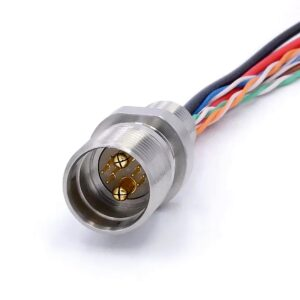
\includegraphics[height=1.7cm, keepaspectratio]{bluetrail_cobalt.jpg}
        \hspace{0.2cm}
        
\includegraphics[height=1.7cm, keepaspectratio]{bluetrail_cobalt_pair.png}
      \end{center}
      \vspace{-0.2em}
      \begin{block}{\tech{Blue Trail Engineering --- Série Cobalt}}
        \scriptsize
        \textbf{\textit{Embase M10 compacte, PEEK / Inox 316, 600\,m (60\,bar)}}\\[0.3em]
        \begin{itemize}\setlength{\itemsep}{1pt}\setlength{\parskip}{0pt}
          \item \textbf{Compatibilité native BlueRobotics} : filetage \textbf{M10} (Cobalt 10), remplace directement un WetLink sans usinage !
          \item Coque inox 316L, inserts PEEK rigides, contacts or.
          \item 3 à 8 pins (M10) et jusqu'à 12 pins / Ethernet (Cobalt 14, M14).
        \end{itemize}
      \end{block}
    \end{column}

    \begin{column}{0.48\textwidth}
      \begin{center}
        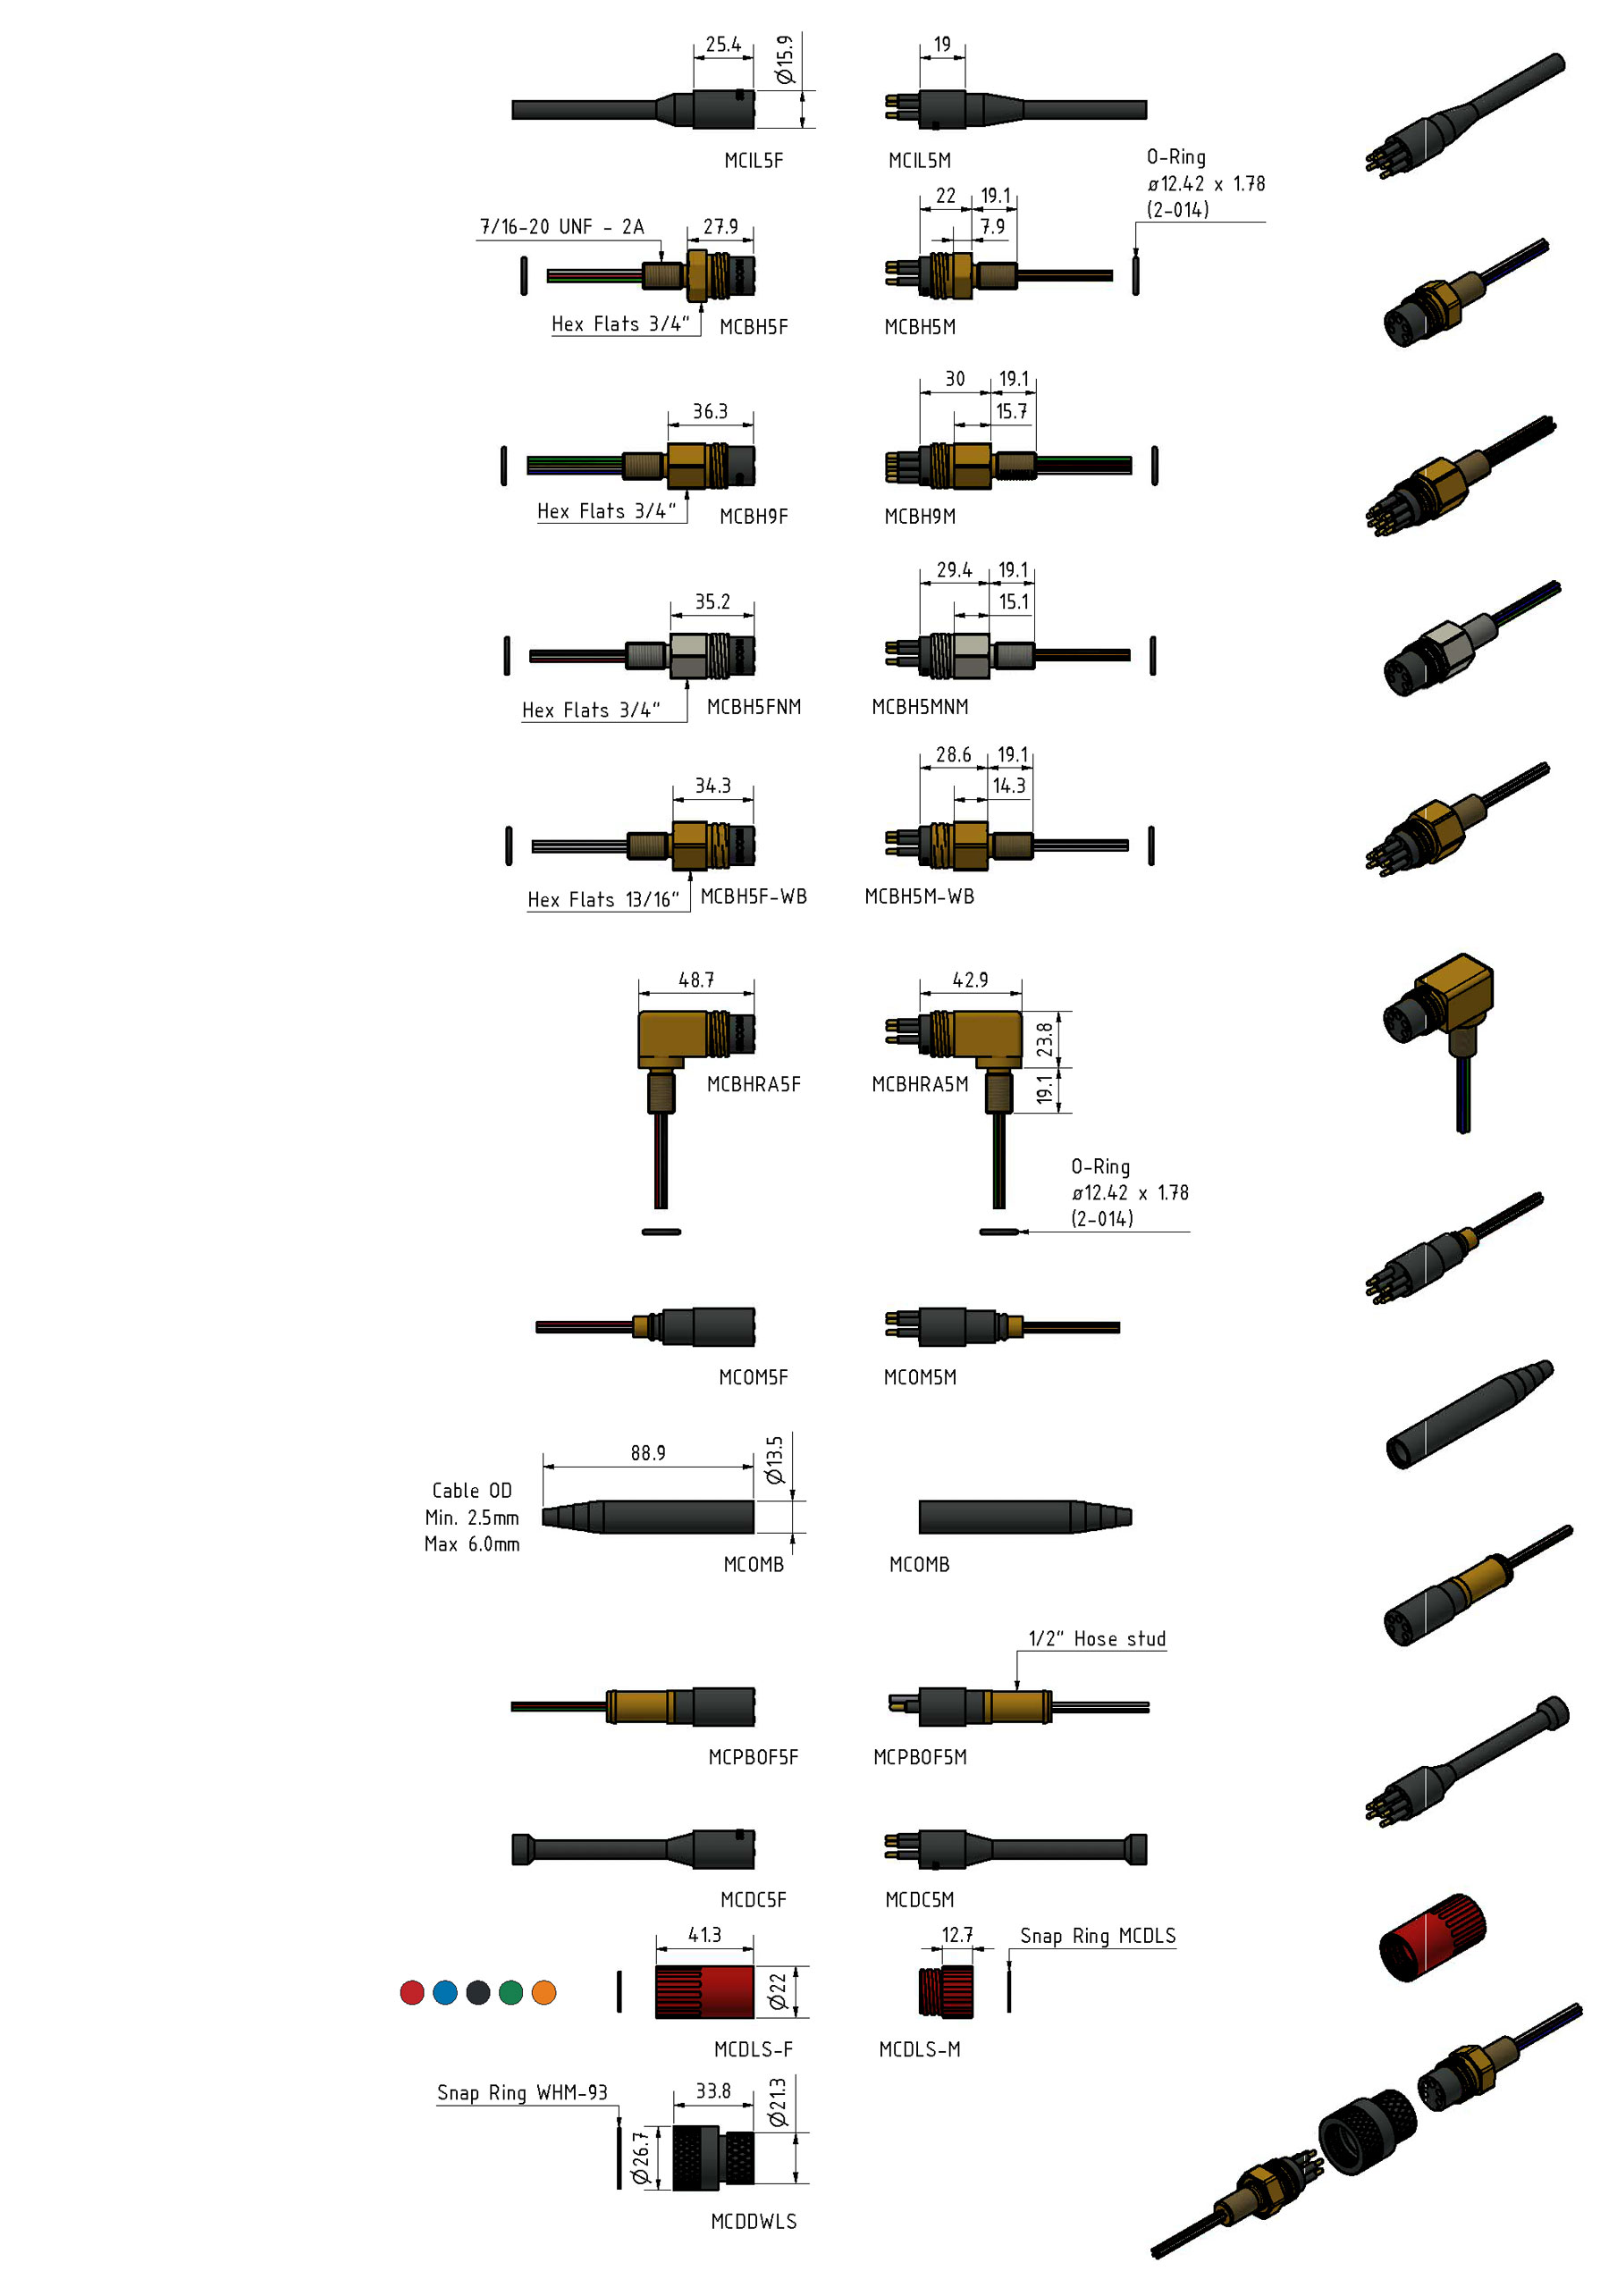
\includegraphics[height=1.7cm, keepaspectratio]{subconn_micro_circular.jpg}
      \end{center}
      \vspace{-0.2em}
      \begin{block}{\tech{SubConn (MacArtney) --- Micro Circular}}
        \scriptsize
        \textbf{\textit{Standard mondial offshore \& océanographie, néoprène}}\\[0.3em]
        \begin{itemize}\setlength{\itemsep}{1pt}\setlength{\parskip}{0pt}
          \item \textbf{Standard historique de l'industrie} : éprouvé depuis plus de 40 ans (Ifremer, navires océanographiques).
          \item Corps surmoulé néoprène souple, bague de verrouillage (*locking sleeve*), haute résistance mécanique.
          \item 2 à 21 contacts, haute tension ($600\,\text{V}$, $10\text{--}15\,\text{A}$).
        \end{itemize}
      \end{block}
    \end{column}
  \end{columns}
\end{frame}

\begin{frame}{2.6b Typologie Opérationnelle : Connectique Dry-Mate vs Wet-Mate}
  \begin{columns}[T]
    \begin{column}{0.49\textwidth}
      \begin{block}{\succw{1. Connecteurs Dry-Mate (Standard Drone)}}
        \scriptsize
        \begin{itemize}
          \item \textbf{Principe} : accouplement et verrouillage effectués \textbf{au sec obligatoirement} sur le pont avant immersion.
          \item Enduction d'un très léger film de graisse silicone sur les fiches.
          \item Étanchéité parfaite jusqu'à 600--2000 m une fois verrouillé.
          \item \succw{Économique, ultra-fiable} et parfaitement adapté aux ROVs/AUVs de laboratoire (Cobalt, SubConn).
        \end{itemize}
      \end{block}
    \end{column}

    \begin{column}{0.49\textwidth}
      \begin{alertblock}{2. Connecteurs Wet-Mate (Haute Technicité)}
        \scriptsize
        \begin{itemize}
          \item \textbf{Principe} : connectable et déconnectable \textbf{directement sous l'eau} en pleine immersion.
          \item Bain d'huile diélectrique interne et membranes racleuses chassant l'eau de mer salée lors de l'enfichage.
          \item \alertw{Extrêmement onéreux} ($>3\,000$ à $8\,000$ € par connecteur).
          \item Réservé aux observatoires fond de mer câblés (EMSO, KM3NeT) et stations d'accueil AUV sous-marines.
        \end{itemize}
      \end{alertblock}
    \end{column}
  \end{columns}
\end{frame}

\begin{frame}{2.7 Gestion de la Pression Caisson : Vents, PRV \& Pompes à Vide}
  \begin{columns}[T]
    \begin{column}{0.32\textwidth}
      \begin{center}
        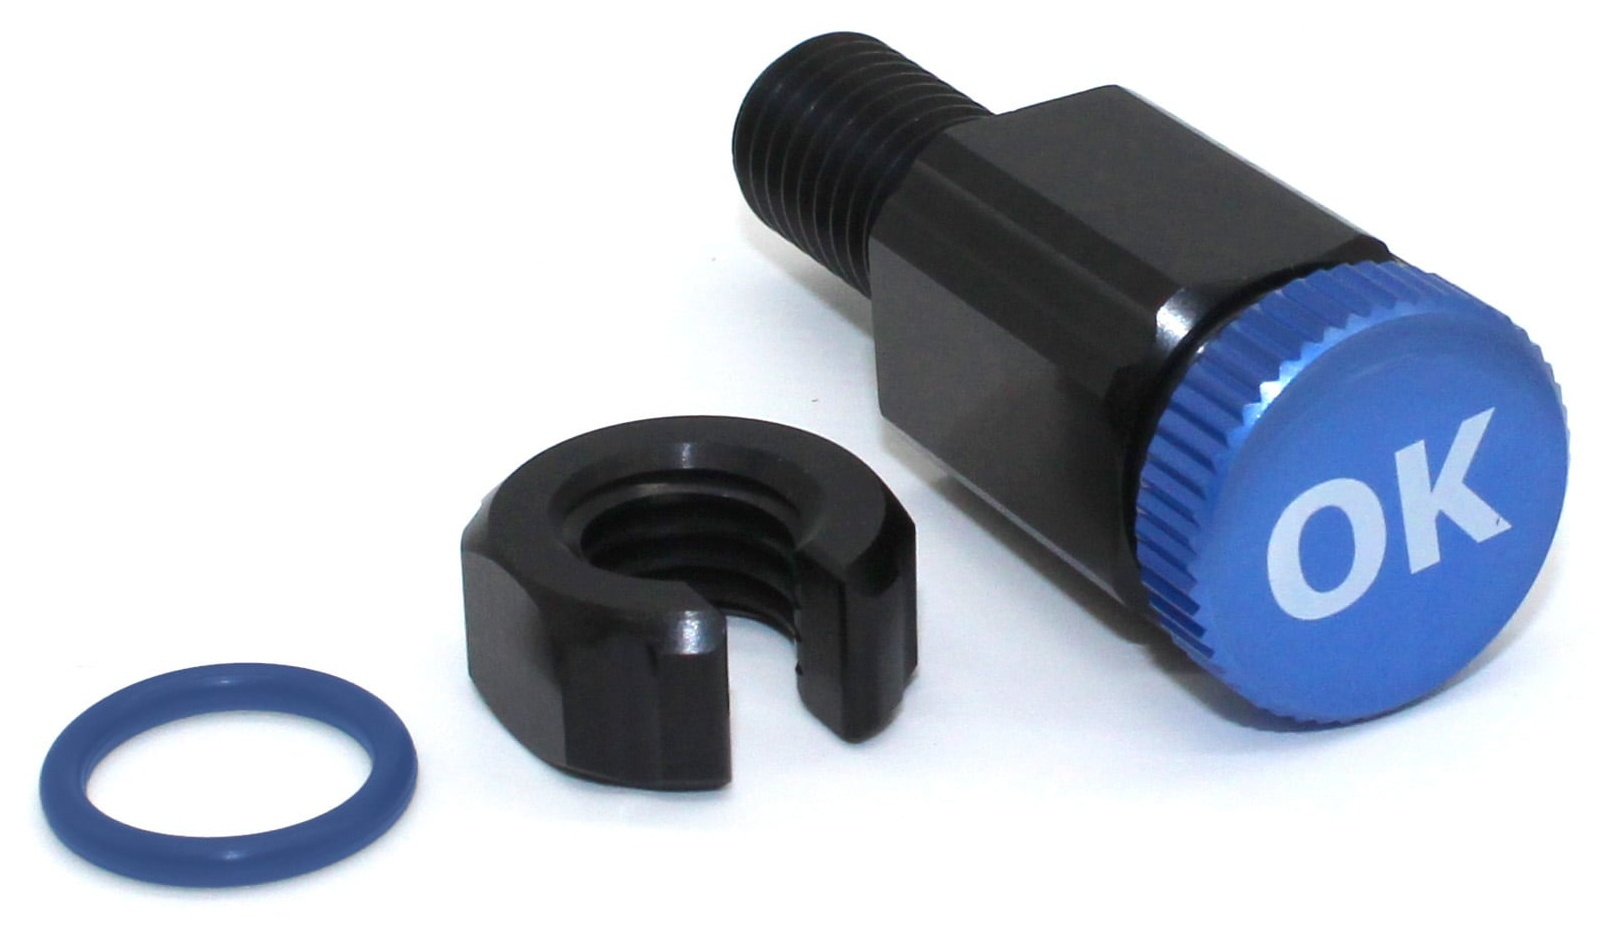
\includegraphics[height=1.35cm, keepaspectratio]{vent_plug_clean.jpg}\\
        \vspace{0.1em}
        \tech{Enclosure Vent and Plug}\\
        \footnotesize\textbf{Bouchon d'Évent M10}
      \end{center}
      \scriptsize
      \begin{itemize}\setlength{\itemsep}{1pt}\setlength{\parskip}{0pt}
        \item \textbf{Équilibrage de pression} : dévissage manuel partiel pour « casser le vide » sans forcer sur les portées ni abîmer les joints.
        \item \textbf{Accès direct sans outil} : bouchon moleté avec double joint torique pour maintenance rapide sur le pont.
        \item \textbf{Port de test dédié} : reçoit l'embout étanche pour le tirage au vide terrain.
      \end{itemize}
    \end{column}

    \begin{column}{0.32\textwidth}
      \begin{center}
        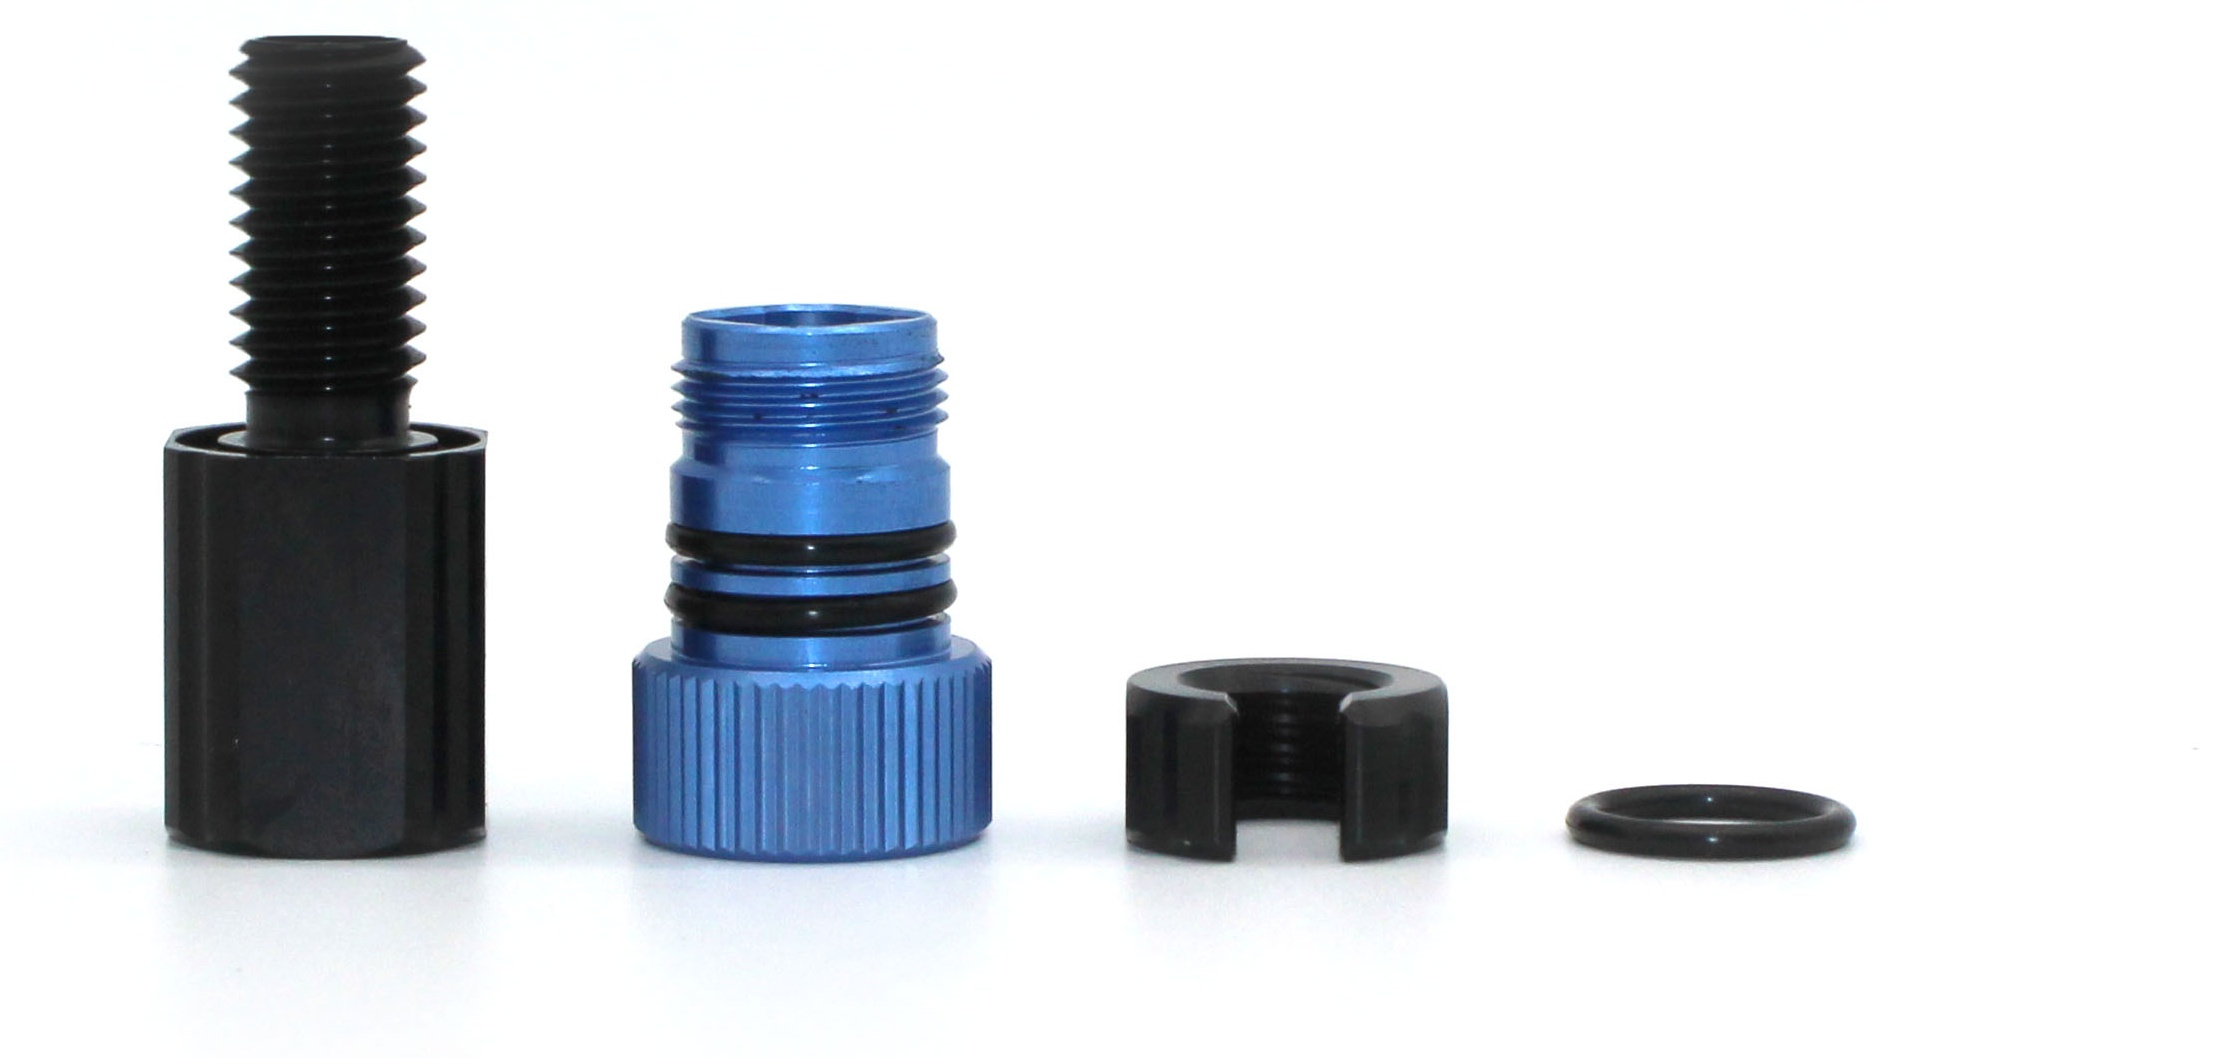
\includegraphics[height=1.35cm, keepaspectratio]{pressure_relief_valve_clean.jpg}\\
        \vspace{0.1em}
        \alertw{Pressure Relief Valve (PRV)}\\
        \footnotesize\textbf{Soupape de Surpression M10}
      \end{center}
      \scriptsize
      \begin{itemize}\setlength{\itemsep}{1pt}\setlength{\parskip}{0pt}
        \item \textbf{Sécurité passive critique} : obligatoire pour tout caisson abritant des batteries \textbf{Li-Ion / LiPo}.
        \item \textbf{Dégazage \& emballement} : évacuation automatique de surpression ($>30\text{--}50\,\text{kPa}$) évitant l'effet « missile » (éjection brutale de flasque).
        \item \textbf{Clapet taré à ressort} : purge les gaz et se referme immédiatement pour préserver l'étanchéité à l'eau.
      \end{itemize}
    \end{column}

    \begin{column}{0.32\textwidth}
      \begin{center}
        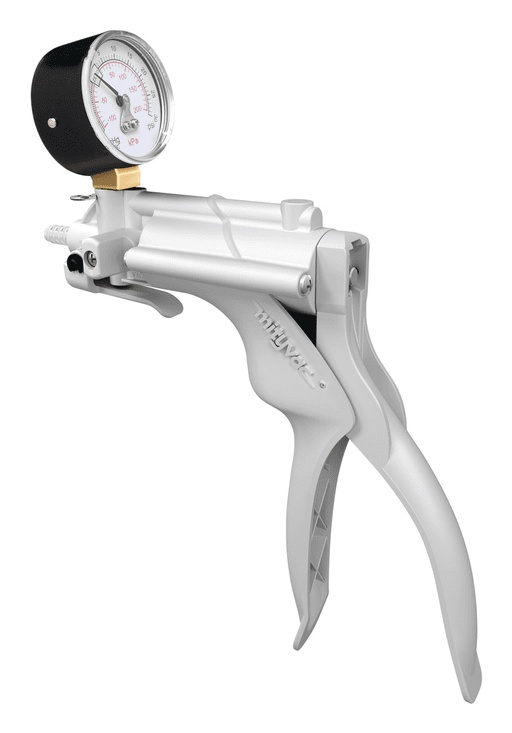
\includegraphics[height=1.5cm, keepaspectratio]{vacuum_pump_clean.jpg}\\
        \vspace{0.1em}
        \succw{Pompe Manuelle à Vide}\\
        \footnotesize\textbf{Testeur de Dépression Terrain}
      \end{center}
      \scriptsize
      \begin{itemize}\setlength{\itemsep}{1pt}\setlength{\parskip}{0pt}
        \item \textbf{Tirage au vide pré-vol} : création d'une dépression relative de \succw{$\mathbf{-0.5\,\text{bar}}$} pour valider l'étanchéité.
        \item \textbf{Manomètre} : détection des micro-fuites sur 15 min.
        \item \textbf{Précharge mécanique} : plaque et verrouille fermement les flasques avant contact avec l'eau.
      \end{itemize}
    \end{column}
  \end{columns}
\end{frame}

\begin{frame}{2.7b Validation Pré-Vol : Le Test de Vide Terrain (Vacuum Test)}
  \begin{alertblock}{La règle d'or absolue avant chaque mise à l'eau}
    Ne jamais immerger un caisson sans avoir validé son étanchéité par dépression.
  \end{alertblock}

  \begin{columns}[T]
    \begin{column}{0.54\textwidth}
      \textbf{Procédure opératoire de terrain} :
      \begin{enumerate}\setlength{\itemsep}{2pt}
        \item Visser l'adaptateur \tech{Vacuum Plug} sur l'évent M10 du caisson.
        \item Raccorder la \tech{pompe à dépression} équipée d'un manomètre de précision.
        \item Pomper pour descendre la pression interne à \succw{$\mathbf{-0.5\,\text{bar}}$ (50 kPa sous le vide relatif)}.
        \item Relever la pression après \textbf{10 minutes} et \textbf{15 minutes} en la lisant sur le manomètre.
        \item Si la pression remonte : \alertw{fuite détectée !} Ne pas plonger.
      \end{enumerate}
    \end{column}

    \begin{column}{0.44\textwidth}
      \begin{center}
        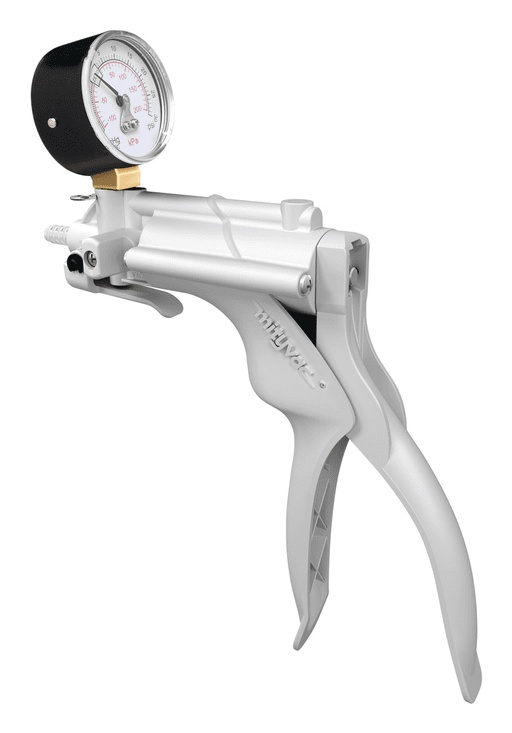
\includegraphics[height=1.9cm, keepaspectratio]{vacuum_pump_clean.jpg}
        \hspace{0.2cm}
        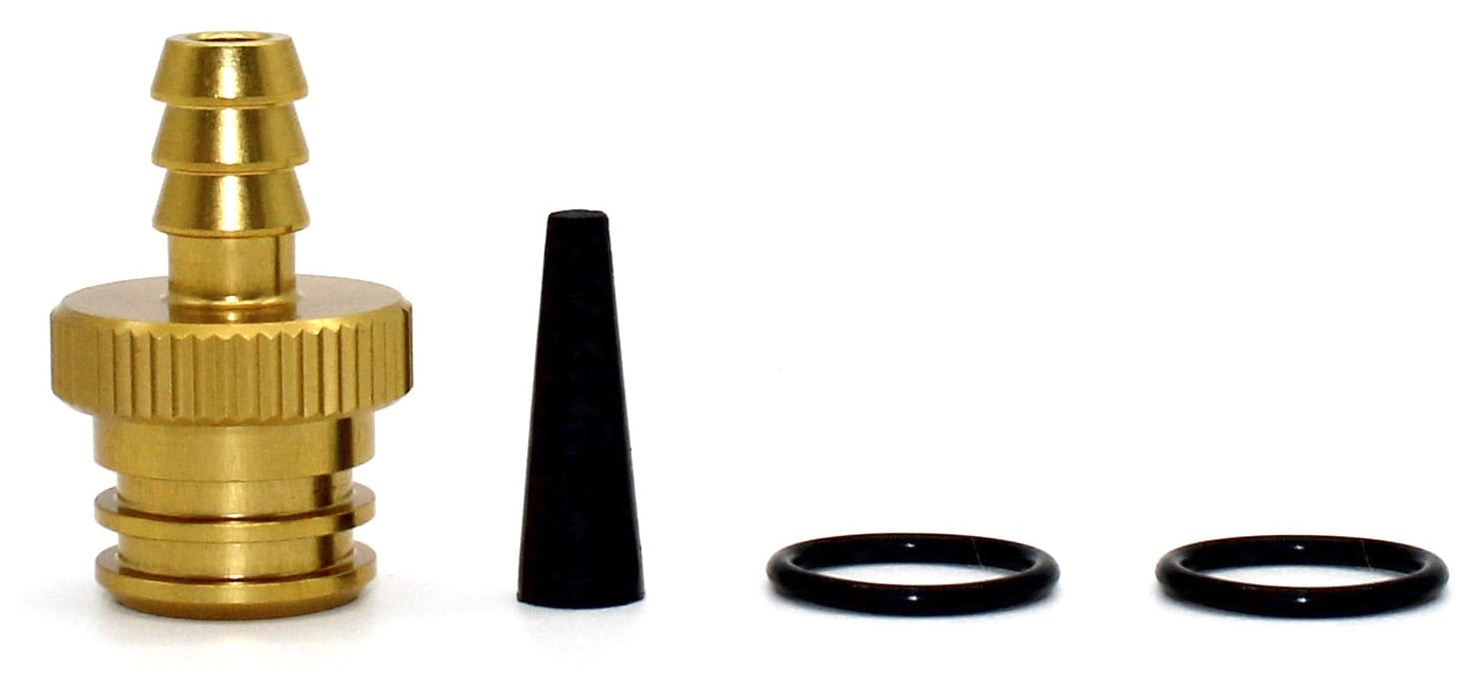
\includegraphics[height=1.3cm, keepaspectratio]{vacuum_plug_clean.jpg}\\
        \vspace{0.1em}
        \tiny\textit{Kit de test à dépression : pompe manuelle \& embout d'évent}
      \end{center}
      \vspace{-0.2em}
      \begin{block}{Causes typiques de fuite}
        \scriptsize
        \begin{itemize}\setlength{\itemsep}{1pt}
          \item Un cheveu ou un grain de sable sur le joint torique.
          \item Excès de graisse silicone ayant piégé une impureté.
          \item Pénétrateur WetLink ou embase connecteur mal serrée sur la flasque.
        \end{itemize}
      \end{block}
    \end{column}
  \end{columns}
\end{frame}

\begin{frame}{2.8 Conception d'un Vecteur de Surface : Le BlueBoat (ASV)}
  \begin{columns}[c]
    \begin{column}{0.42\textwidth}
      \begin{center}
        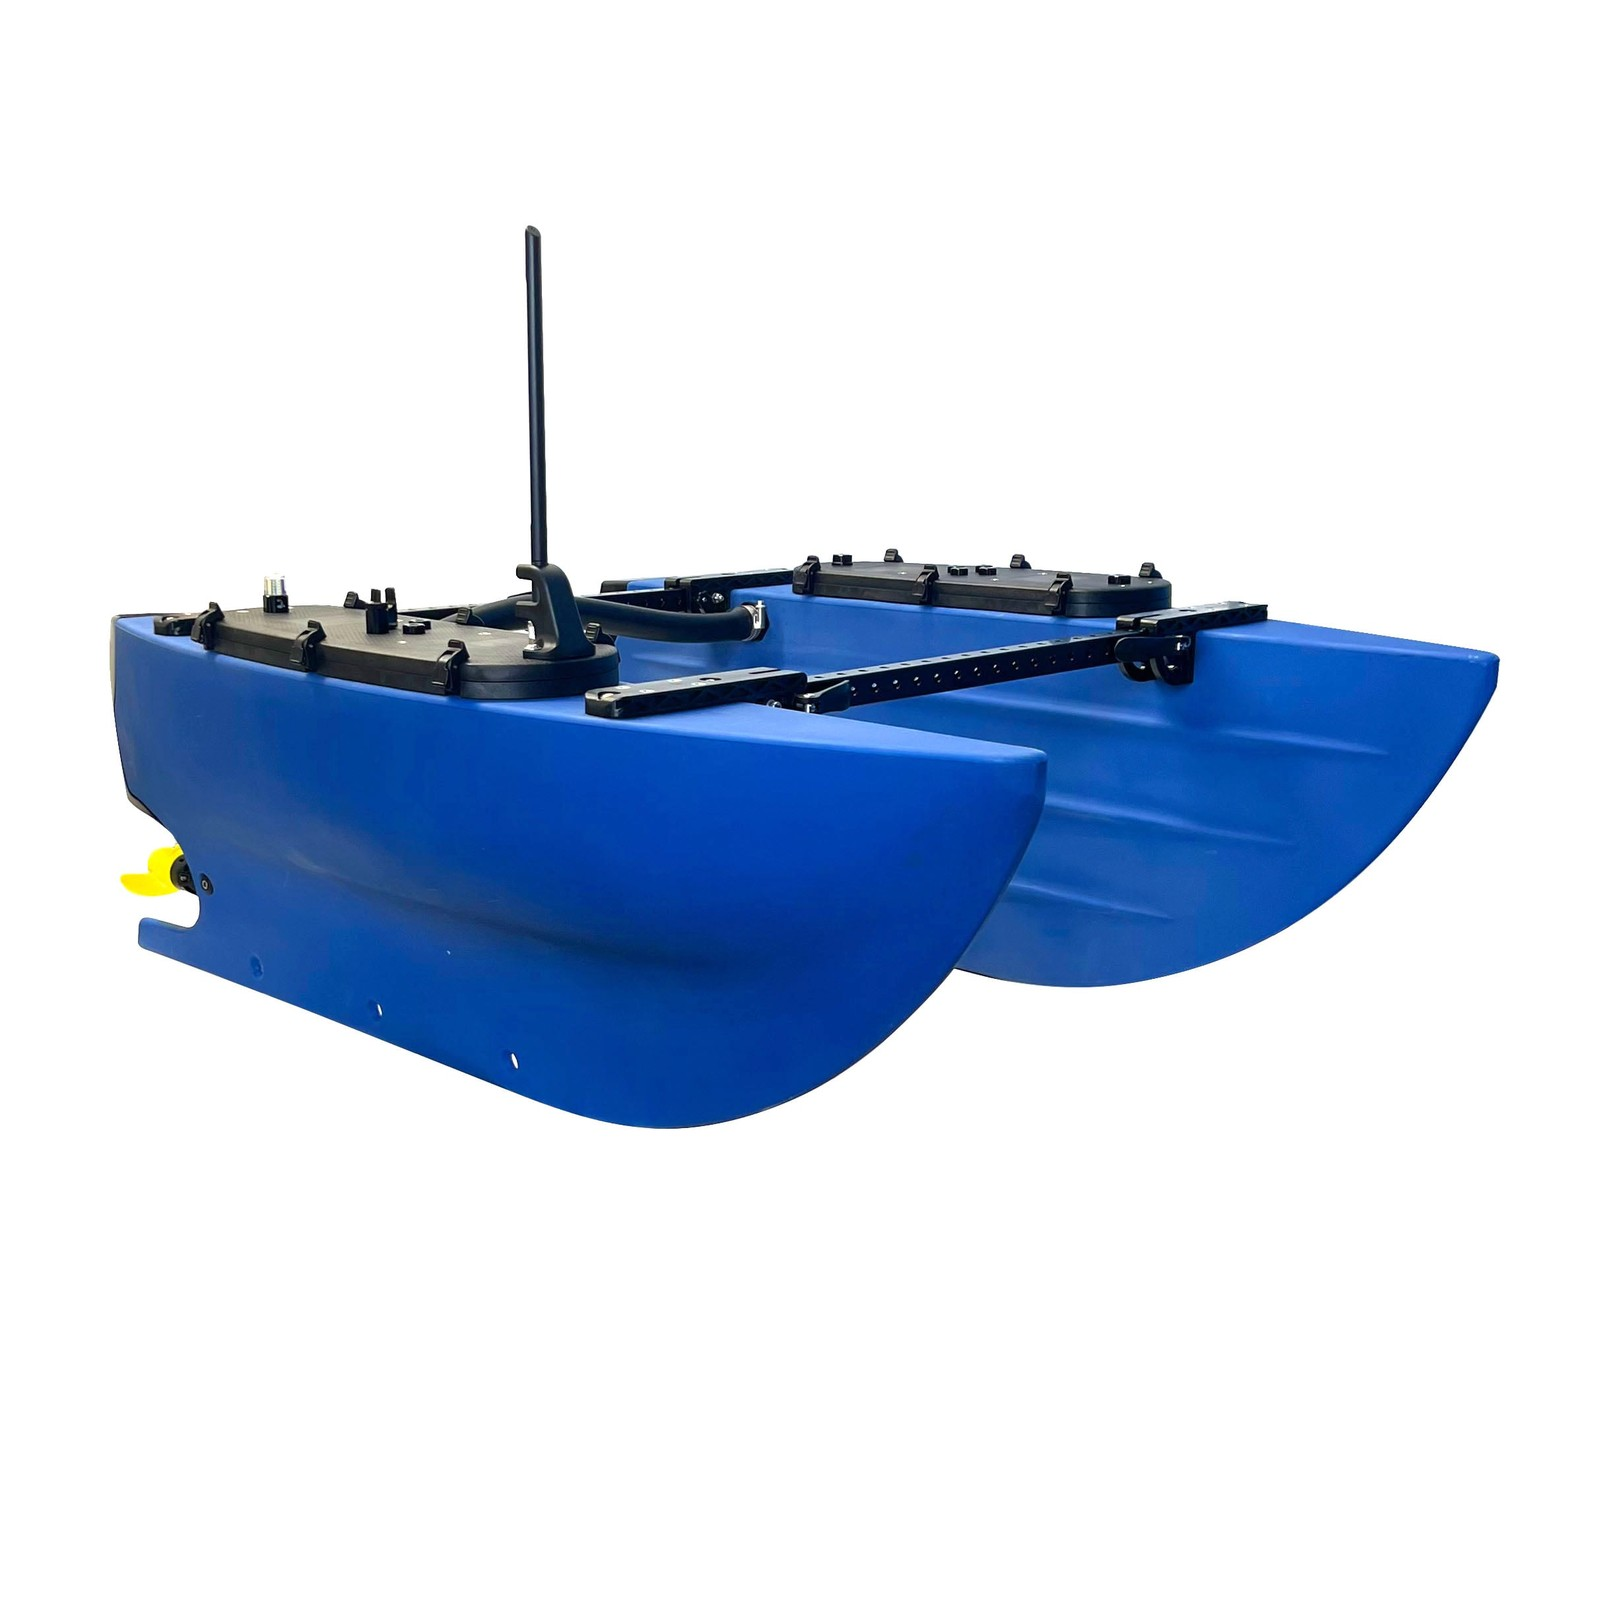
\includegraphics[width=\textwidth, height=4.2cm, keepaspectratio]{blueboat.jpg}\\
        \vspace{0.2em}
        \small\textbf{BlueBoat} (BlueRobotics)\\
        \scriptsize\textit{Catamaran PEHD rotomoulé, 2x T200, baie centrale d'instruments}
      \end{center}
    \end{column}

    \begin{column}{0.56\textwidth}
      \textbf{Architecture \& Caractéristiques} :
      \scriptsize
      \begin{itemize}
        \item \textbf{Coque catamaran} en polyéthylène rotomoulé : quasi-insensible aux impacts contre roches et quais.
        \item Tirant d'eau très faible ($\approx 15\,\text{cm}$) pour lagunes, estuaires et rivières.
        \item \textbf{Propulsion différentielle (*skid-steering*)} : 2 propulseurs T200 avec pâles anti-algues.
        \item \textbf{Baie centrale ouverte} : barres profilées pour fixer ADCP, échosondeurs, sondes CTD.
        \item Pliable sans outil pour transport en voiture.
      \end{itemize}

      \vspace{0.3em}
      \begin{block}{Atouts pour la Recherche}
        \scriptsize
        \begin{itemize}
          \item Autonomie : jusqu'à \textbf{8 à 10 heures} de levé continu ($14.8\,\text{V}$ $30\text{Ah}$).
          \item GNSS : localisation metrique.
          \item Télémétrie WiFi longue portée ($>500\,\text{m}$) ou lien 4G.
        \end{itemize}
      \end{block}
    \end{column}
  \end{columns}
\end{frame}

\begin{frame}{2.8b Architecture Interne du BlueBoat : Électronique \& Propulsion}
  \centering
  \begin{tikzpicture}[
    scale=0.74, every node/.style={transform shape},
    box/.style={rounded corners=3pt, align=center, line width=0.8pt},
    pwr/.style={line width=1.6pt, OceanCoral, -{Latex[length=2.0mm]}},
    pwr5v/.style={line width=1.1pt, OceanCoral!85!black, dashed, -{Latex[length=1.7mm]}},
    sig/.style={line width=1.0pt, OceanCyan!90!black, dashed, -{Latex[length=1.7mm]}},
    net/.style={line width=1.3pt, OceanLight, <->, >=Latex},
    mot/.style={line width=1.6pt, DarkSlate, -{Latex[length=2.0mm]}},
    wlp/.style={draw=OceanDeep, fill=yellow!45, line width=1.1pt, rounded corners=2pt, font=\bfseries, align=center},
    badge/.style={fill=white, rounded corners=2pt, inner sep=1.1pt, font=\tiny\bfseries}
  ]

    % 1. Zone Coques étanches (Hulls)
    \fill[OceanGray!35, rounded corners=6pt] (-0.45, 0.32) rectangle (10.35, 5.05);
    \draw[OceanMedium, line width=1.4pt, rounded corners=6pt] (-0.45, 0.32) rectangle (10.35, 5.05);
    
    % Titre bandeau de la coque étanche
    \node[anchor=south west, fill=OceanMedium, text=white, font=\tiny\bfseries, rounded corners=2pt, inner sep=2.5pt] at (-0.20, 5.05) {%
      ~COQUE ÉTANCHE DU BLUEBOAT (PEHD rotomoulé --- 1\,atm sec)~%
    };

    % 2. Zone Extérieure (Milieu aquatique)
    \fill[OceanCyan!8, rounded corners=6pt] (10.75, 0.32) rectangle (14.55, 5.05);
    \draw[OceanCyan!60, dashed, line width=1.2pt, rounded corners=6pt] (10.75, 0.32) rectangle (14.55, 5.05);
    
    % Titre bandeau milieu extérieur
    \node[anchor=south, fill=OceanCyan!85!black, text=white, font=\tiny\bfseries, rounded corners=2pt, inner sep=2.5pt] at (12.65, 5.05) {%
      ~MILIEU MARIN EXTÉRIEUR (Immergé)~%
    };
    \node[anchor=north, font=\tiny\itshape, text=OceanCyan!85!black] at (12.65, 4.95) {(Eau de mer / Pression hydrostatique)};

    % 3. Calcul, GNSS & Télécoms (x = 0.40 à 2.10)
    \node[box, draw=OceanDeep, fill=white, minimum width=1.45cm, minimum height=0.72cm] (gnss) at (0.40, 3.90) {
      \textbf{\scriptsize GNSS}
    };

    \node[box, draw=OceanLight, fill=OceanLight!15, minimum width=1.45cm, minimum height=0.72cm] (wifi) at (2.10, 3.90) {
      \textbf{\scriptsize Routeur WiFi}\\
      \tiny Liaison sol $2.4/5\,$G
    };

    \node[box, draw=OceanDeep, fill=OceanDeep!15, minimum width=2.5cm, minimum height=0.72cm] (rpi) at (1.25, 2.40) {
      \textbf{\scriptsize Raspberry Pi 4}\\
      \tiny Compagnon (BlueOS)
    };

    \node[box, draw=OceanCyan, fill=OceanCyan!15, minimum width=2.5cm, minimum height=0.72cm] (nav) at (1.25, 0.95) {
      \textbf{\scriptsize Navigator (HAT)}\\
      \tiny Autopilote ArduRover
    };

    % Antennes sur le pont (vers le ciel)
    \draw[line width=1.2pt, OceanDeep] (gnss.north) -- ++(0, 0.38);
    \node[anchor=south, badge, draw=OceanDeep!60, fill=white, text=OceanDeep] at ($(gnss.north)+(0, 0.38)$) {Antenne GNSS};

    \draw[line width=1.2pt, OceanLight] (wifi.north) -- ++(0, 0.38);
    \node[anchor=south, badge, draw=OceanLight!60, fill=OceanLight!10, text=OceanLight] at ($(wifi.north)+(0, 0.38)$) {Antenne WiFi};

    % Liaisons internes Calcul (Gauche) : strictement verticales
    \draw[sig, OceanDeep, line width=1.1pt] (gnss.south) -- ($(rpi.north)-(0.85, 0)$) 
      node[midway, badge, draw=OceanDeep!40, text=OceanDeep]{USB/NMEA};
    \draw[net] (wifi.south) -- ($(rpi.north)+(0.85, 0)$) 
      node[midway, badge, draw=OceanLight!40, text=OceanLight]{Ethernet};
    \draw[net, OceanCyan, line width=1.4pt] (rpi) -- (nav) 
      node[midway, badge, draw=OceanCyan!40, text=OceanCyan!90!black]{Bus HAT (GPIO)};

    % 4. Énergie (Colonne 2, x = 4.75)
    \node[box, draw=OceanCoral, fill=OceanCoral!15, minimum width=2.5cm, minimum height=0.75cm] (bat) at (4.75, 3.90) {
      \textbf{\scriptsize Batteries Li-Ion}\\
      \tiny $14.8\,\text{V}$ (4S, $18\text{--}30\,\text{Ah}$)
    };

    \node[box, draw=OceanCoral!85!black, fill=white, minimum width=2.6cm, minimum height=0.90cm] (pdb) at (4.75, 2.40) {
      \textbf{\scriptsize Carte Distribution (PDB)}\\
      \tiny Shunt $U/I$ \& Régulateurs BEC
    };

    % Liaison Batterie vers PDB
    \draw[pwr, line width=2.0pt] (bat) -- (pdb) node[midway, badge, draw=OceanCoral!40, text=OceanCoral!90!black]{14.8\,V (VBAT)};

    % Alimentations régulées depuis PDB
    % 5V BEC vers RPi : horizontal direct à y = 2.22
    \draw[pwr5v] ($(pdb.west)-(0, 0.18)$) -- ($(rpi.east)-(0, 0.18)$) 
      node[midway, badge, draw=OceanCoral!40, text=OceanCoral!85!black]{5\,V BEC};
    
    % 12V vers WiFi : sort à y = 2.62, monte par x = 3.15 dégagé
    \draw[pwr5v] ($(pdb.west)+(0, 0.22)$) -- (3.15, 2.62) -- (3.15, 3.90) -- (wifi.east);
    \node[badge, draw=OceanCoral!40, text=OceanCoral!85!black] at (3.15, 3.25) {12\,V};

    % 5. Variateurs ESC (Colonne 3, x = 7.95)
    \node[box, draw=OceanGreen, fill=OceanGreen!15, minimum width=2.0cm, minimum height=0.75cm] (esc_b) at (7.95, 3.90) {
      \textbf{\scriptsize ESC Bâbord}\\
      \tiny Basic ESC (30\,A)
    };

    \node[box, draw=OceanGreen, fill=OceanGreen!15, minimum width=2.0cm, minimum height=0.75cm] (esc_t) at (7.95, 0.95) {
      \textbf{\scriptsize ESC Tribord}\\
      \tiny Basic ESC (30\,A)
    };

    % Alimentation puissance 14.8V PDB vers ESCs (Couloir x in [6.05, 6.95])
    % Vers ESC Bâbord (monte par x = 6.45, entre par le haut à y = 4.05)
    \draw[pwr] ($(pdb.east)+(0, 0.20)$) -- (6.45, 2.60) -- (6.45, 4.05) -- ($(esc_b.west)+(0, 0.15)$);
    \node[badge, draw=OceanCoral!40, text=OceanCoral!90!black] at (6.45, 3.35) {14.8\,V};

    % Vers ESC Tribord (descend par x = 6.45, entre par le haut à y = 1.10)
    \draw[pwr] ($(pdb.east)-(0, 0.20)$) -- (6.45, 2.20) -- (6.45, 1.10) -- ($(esc_t.west)+(0, 0.15)$);
    \node[badge, draw=OceanCoral!40, text=OceanCoral!90!black] at (6.45, 1.65) {14.8\,V};

    % Commandes PWM Moteurs (Nav vers ESCs) : aucun croisement, cheminements strictement horizontaux puis verticaux
    % PWM Tribord : direct horizontalement sous la PDB à y = 0.80
    \draw[sig] ($(nav.east)-(0, 0.15)$) -- ($(esc_t.west)-(0, 0.15)$)
      node[pos=0.68, badge, draw=OceanCyan!50, text=OceanCyan!90!black]{PWM Tribord (Servo 2)};

    % PWM Bâbord : horizontal direct à y = 1.20 puis monte par x = 6.75 (entre sous la ligne 14.8V à y = 3.75)
    \draw[sig] ($(nav.east)+(0, 0.25)$) -- (6.75, 1.20) 
      node[pos=0.45, badge, draw=OceanCyan!50, text=OceanCyan!90!black]{PWM Bâbord (Servo 1)}
      -- (6.75, 3.75) -- ($(esc_b.west)-(0, 0.15)$);

    % 6. Pénétrateurs WLP (Frontière de paroi, x = 10.35)
    \node[wlp, minimum width=1.15cm, minimum height=0.62cm] (wlp_b) at (10.35, 3.90) {
      \textbf{\tiny WLP}\\
      \tiny M10
    };

    \node[wlp, minimum width=1.15cm, minimum height=0.62cm] (wlp_t) at (10.35, 0.95) {
      \textbf{\tiny WLP}\\
      \tiny M10
    };

    % Encadré d'explication des Pénétrateurs WLP (centré sur la paroi)
    \node[badge, draw=OceanDeep, fill=yellow!25, line width=0.8pt, align=center, text=OceanDeep] (wlp_info) at (10.35, 2.40) {%
      \textbf{\tiny Traversée Étanche}\\[-0.2ex]
      \tiny Pénétrateurs WetLink\\[-0.2ex]
      \tiny (\textit{Écrou M10 étanche})%
    };
    \draw[line width=0.7pt, OceanDeep, ->] (wlp_info.north) -- (wlp_b.south);
    \draw[line width=0.7pt, OceanDeep, ->] (wlp_info.south) -- (wlp_t.north);

    % 7. Propulseurs T200 (Extérieur, x = 12.65)
    \node[box, draw=OceanDeep, fill=OceanDeep!18, minimum width=2.4cm, minimum height=0.85cm] (t200_b) at (12.65, 3.90) {
      \textbf{\scriptsize Propulseur T200}\\
      \tiny Moteur Bâbord (\textit{Port})
    };

    \node[box, draw=OceanDeep, fill=OceanDeep!18, minimum width=2.4cm, minimum height=0.85cm] (t200_t) at (12.65, 0.95) {
      \textbf{\scriptsize Propulseur T200}\\
      \tiny Moteur Tribord (\textit{Starboard})
    };

    % Traversée de paroi étanche WLP vers T200 (Câbles moteurs triphasés)
    \draw[mot] (esc_b.east) -- (wlp_b.west) node[midway, badge, draw=DarkSlate!30, text=DarkSlate]{3 phases};
    \draw[mot] (wlp_b.east) -- (t200_b.west);

    \draw[mot] (esc_t.east) -- (wlp_t.west) node[midway, badge, draw=DarkSlate!30, text=DarkSlate]{3 phases};
    \draw[mot] (wlp_t.east) -- (t200_t.west);

    % Légende synthétique en bas
    \node[anchor=west, font=\tiny, text=DarkSlate] at (-0.35, 0.08) {%
      \textbf{Flux :}~
      \textcolor{OceanCoral}{\rule[0.5ex]{8pt}{1.8pt}}~\textbf{14.8\,V (VBAT)}\quad
      \textcolor{OceanCoral!85!black}{\textbf{- -}~\textbf{BEC 5V/12V}}\quad
      \textcolor{OceanCyan!90!black}{\textbf{- -}~\textbf{PWM}}\quad
      \textcolor{OceanDeep}{\textbf{- -}~\textbf{USB/NMEA}}\quad
      \textcolor{OceanLight}{\textbf{$\leftrightarrow$}~\textbf{Ethernet/HAT}}\quad
      \textcolor{DarkSlate}{\rule[0.5ex]{8pt}{1.6pt}}~\textbf{Triphasé}%
    };

  \end{tikzpicture}

  \vspace{0.1em}
  \begin{columns}[T, onlytextwidth]
    \begin{column}{0.32\textwidth}
      \begin{block}{\tech{1. Calcul, GNSS \& Sol}}
        \scriptsize
        \textbf{RPi 4} (BlueOS) + \textbf{Navigator} (ArduRover). Le \textbf{GNSS/RTK} assure le cap et positionnement métrique ; le \textbf{routeur WiFi} la liaison sol ($>500\,\text{m}$).
      \end{block}
    \end{column}

    \begin{column}{0.32\textwidth}
      \begin{block}{\succw{2. Puissance \& Distribution}}
        \scriptsize
        \textbf{Batteries Li-Ion} reliées à la \textbf{PDB} : bus forte intensité ($14.8\,\text{V}$) vers ESCs et conversion régulée ($5\,\text{V}$) pour l'électronique.
      \end{block}
    \end{column}

    \begin{column}{0.32\textwidth}
      \begin{block}{\alertw{3. Traversée \& Propulsion}}
        \scriptsize
        Les \textbf{pénétrateurs WetLink (WLP)} assurent l'étanchéité des phases moteurs traversant la coque (\textit{hulls}) vers les \textbf{T200} immergés.
      \end{block}
    \end{column}
  \end{columns}
\end{frame}
\begin{frame}{2.8c Conception d'un Vecteur Sous-Marin : Le BlueROV2 (ROV)}
  \begin{columns}[c]
    \begin{column}{0.42\textwidth}
      \begin{center}
        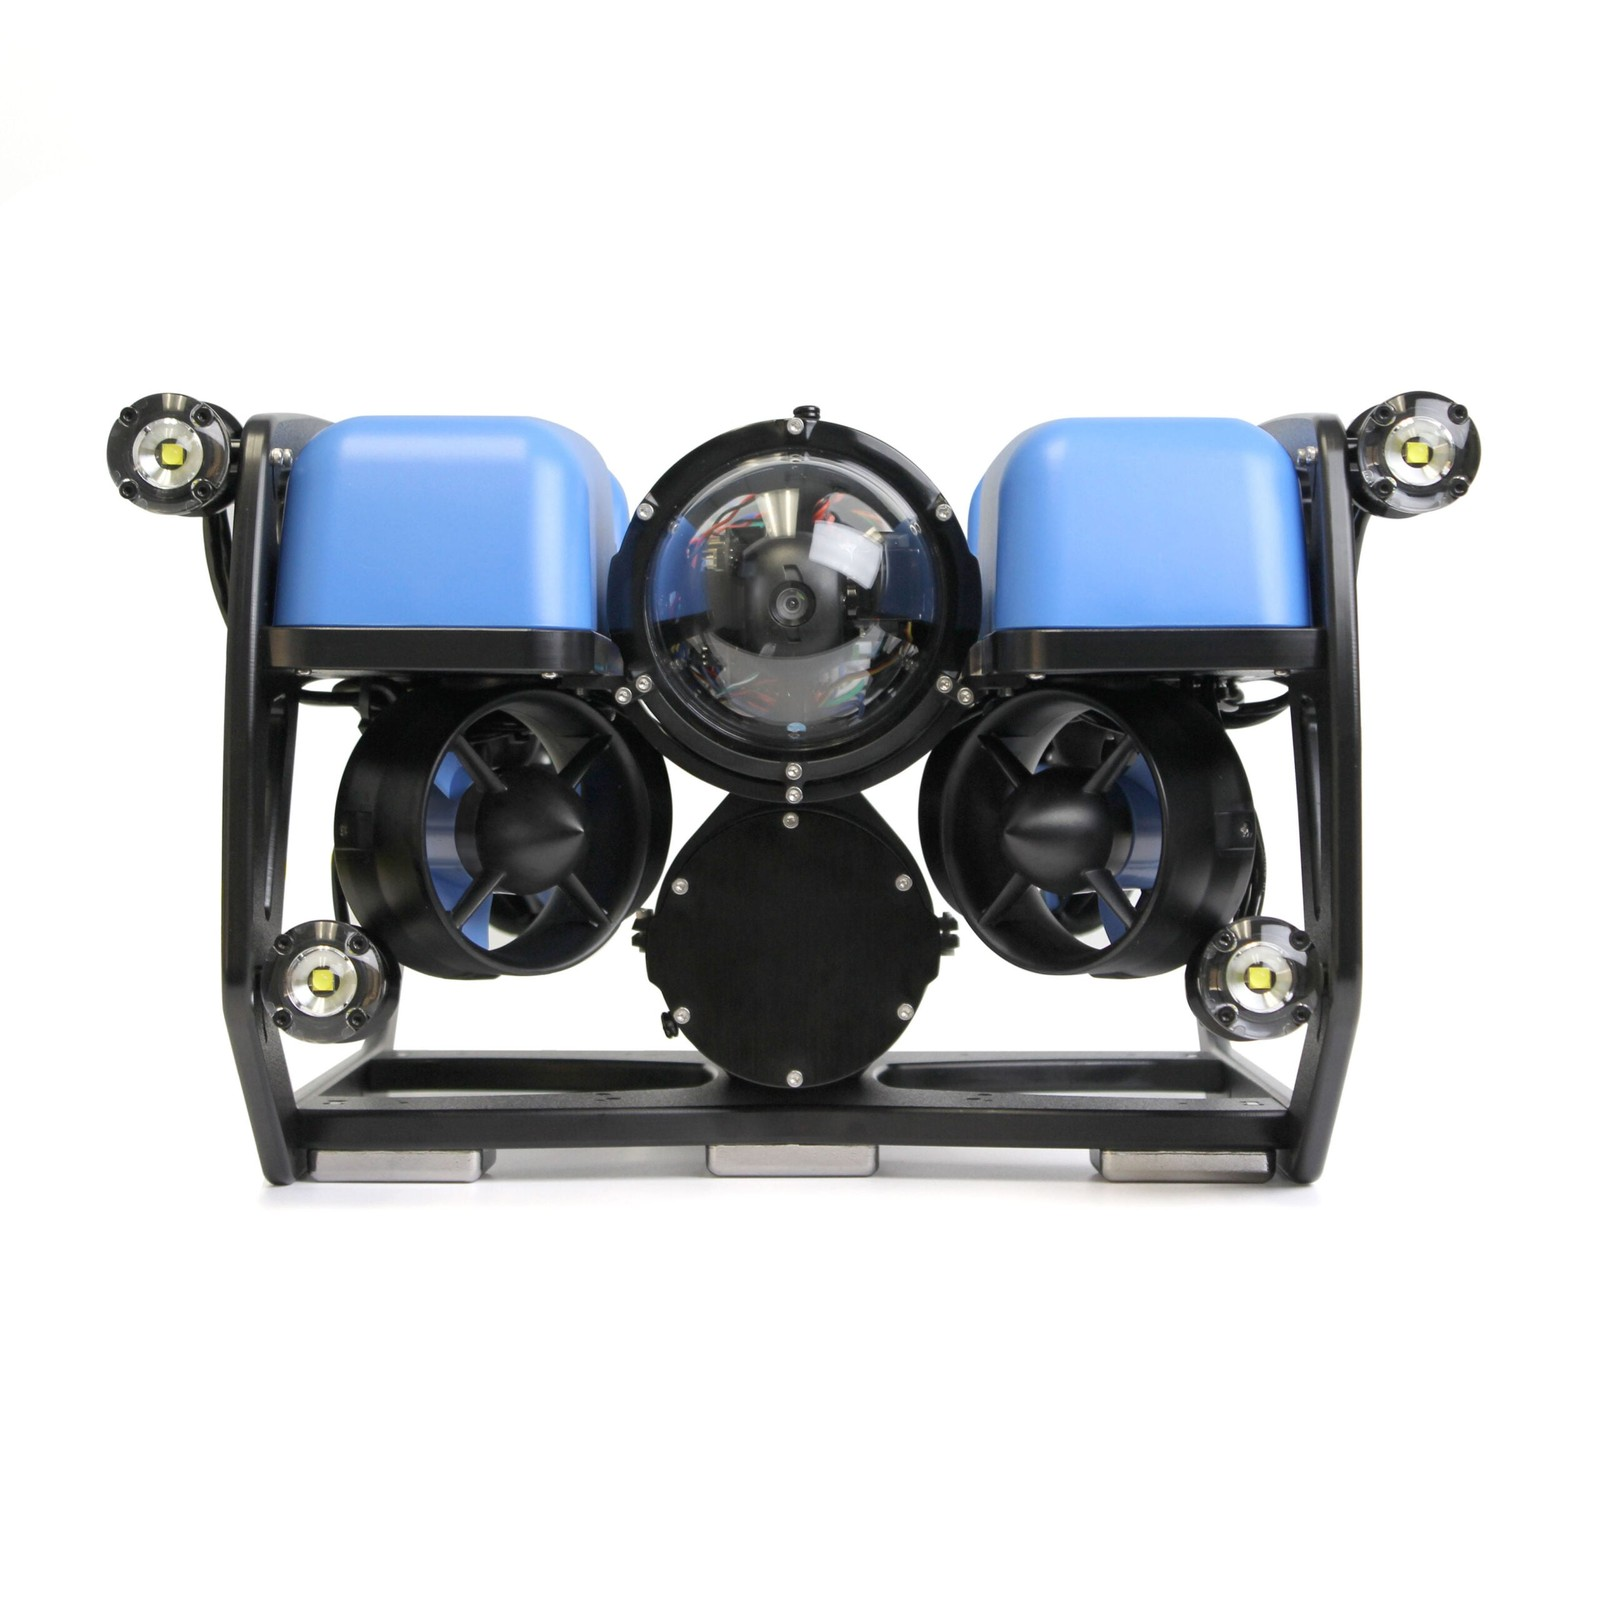
\includegraphics[width=\textwidth, height=4.2cm, keepaspectratio]{bluerov2.jpg}\\
        \vspace{0.2em}
        \small\textbf{BlueROV2} (BlueRobotics)\\
        \scriptsize\textit{Châssis modulaire PEHD, double caisson étanche (4" \& 3"), 6 à 8x T200, ombilical Fathom}
      \end{center}
    \end{column}

    \begin{column}{0.56\textwidth}
      \textbf{Architecture \& Parties Constituantes} :
      \scriptsize
      \begin{itemize}\setlength{\itemsep}{1.5pt}\setlength{\parskip}{0pt}
        \item \textbf{Châssis modulaire en PEHD} : berceau insensible à la corrosion, supportant les blocs de mousse de flottabilité haute ($\overline{BG} > 0$).
        \item \textbf{Double enceinte étanche} : caisson supérieur (tube 4") pour l'électronique \& caisson inférieur (tube 3") pour la batterie.
        \item \textbf{Propulsion vectorisée} : 6 à 8 propulseurs \textbf{T200} (moteurs brushless à rotor noyé) offrant jusqu'à \succw{6 degrés de liberté}.
        \item \textbf{Liaison ombilicale filaire (Tether)} : câble fin à flottabilité neutre transportant le flux réseau haut débit (Fathom-X).
        \item \textbf{Franchissements de flasques} : pénétrateurs \textbf{WetLink (WLP M10)} assurant l'étanchéité jusqu'à $100\text{--}300\,\text{m}$.
      \end{itemize}

      \vspace{0.25em}
      \begin{block}{Atouts pour la Recherche \& l'Observation}
        \scriptsize
        \begin{itemize}\setlength{\itemsep}{1pt}\setlength{\parskip}{0pt}
          \item \textbf{Téléopération temps réel} : flux vidéo HD/4K à faible latence et télémétrie complète sous MAVLink (QGroundControl).
          \item \textbf{Stationnarité parfaite} : tenue de cap et maintien de profondeur automatiques (\textit{Depth Hold} via capteur Bar30).
          \item \textbf{Payload modulaire} : intégration simple de capteurs scientifiques (sonde CTD, sonar Ping360, DVL-A50, balise USBL).
        \end{itemize}
      \end{block}
    \end{column}
  \end{columns}
\end{frame}

\begin{frame}{2.8d Architecture Globale du BlueROV2 : Électronique, Ombilical \& Propulsion}
  \centering
  \begin{tikzpicture}[
    scale=0.72, every node/.style={transform shape},
    box/.style={rounded corners=3pt, align=center, line width=0.8pt},
    pwr/.style={line width=1.6pt, OceanCoral, -{Latex[length=2.0mm]}},
    pwr5v/.style={line width=1.1pt, OceanCoral!85!black, dashed, -{Latex[length=1.7mm]}},
    sig/.style={line width=1.0pt, OceanCyan!90!black, dashed, -{Latex[length=1.7mm]}},
    net/.style={line width=1.3pt, OceanLight, <->, >=Latex},
    mot/.style={line width=1.6pt, DarkSlate, -{Latex[length=2.0mm]}},
    wlp/.style={draw=OceanDeep, fill=yellow!45, line width=1.1pt, rounded corners=2pt, font=\bfseries, align=center},
    badge/.style={fill=white, rounded corners=2pt, inner sep=1.1pt, font=\tiny\bfseries}
  ]

    % 1. Zone Surface / Sol (Topside)
    \fill[OceanGray!35, rounded corners=6pt] (-0.40, 0.70) rectangle (2.30, 5.05);
    \draw[DarkSlate!35, dashed, line width=1.1pt, rounded corners=6pt] (-0.40, 0.70) rectangle (2.30, 5.05);
    \node[anchor=south, fill=DarkSlate, text=white, font=\tiny\bfseries, rounded corners=2pt, inner sep=2.5pt] at (0.95, 5.05) {%
      ~SURFACE (POSTE SOL)~%
    };
    \node[anchor=north, font=\tiny\itshape, text=DarkSlate] at (0.95, 4.95) {(Air / Topside)};

    % 2. Zone Caisson Électronique (Tube 4")
    \fill[OceanGray!35, rounded corners=6pt] (3.90, 0.70) rectangle (11.20, 5.05);
    \draw[OceanMedium, line width=1.4pt, rounded corners=6pt] (3.90, 0.70) rectangle (11.20, 5.05);
    \node[anchor=south west, fill=OceanMedium, text=white, font=\tiny\bfseries, rounded corners=2pt, inner sep=2.5pt] at (4.10, 5.05) {%
      ~CAISSON ÉLECTRONIQUE (Tube 4'' --- Intérieur sec 1\,atm)~%
    };

    % 3. Zone Caisson Batterie (Tube 3")
    \fill[OceanGray!35, rounded corners=6pt] (5.90, -0.80) rectangle (9.50, 0.35);
    \draw[OceanMedium, line width=1.3pt, rounded corners=6pt] (5.90, -0.80) rectangle (9.50, 0.35);
    \node[anchor=north west, font=\tiny\bfseries, text=OceanDeep] at (6.05, 0.30) {Caisson Batterie (Tube 3'' --- $G$ bas)};

    % 4. Zone Milieu Marin Extérieur (Immergé)
    \fill[OceanCyan!8, rounded corners=6pt] (11.60, 0.70) rectangle (15.00, 5.05);
    \draw[OceanCyan!60, dashed, line width=1.2pt, rounded corners=6pt] (11.60, 0.70) rectangle (15.00, 5.05);
    \node[anchor=south, fill=OceanCyan!85!black, text=white, font=\tiny\bfseries, rounded corners=2pt, inner sep=2.5pt] at (13.30, 5.05) {%
      ~MILIEU MARIN EXTÉRIEUR~%
    };
    \node[anchor=north, font=\tiny\itshape, text=OceanCyan!85!black] at (13.30, 4.95) {(Eau de mer / Immersion)};

    % --- Composants Surface / Poste Sol ---
    \node[box, draw=OceanLight, fill=OceanLight!15, minimum width=2.2cm, minimum height=0.75cm] (fxti) at (0.95, 3.90) {
      \textbf{\scriptsize Fathom-X Sol}\\
      \tiny Boîtier FXTI (CPL)
    };

    \node[box, draw=OceanDeep, fill=OceanDeep!10, minimum width=2.2cm, minimum height=0.75cm] (pc) at (0.95, 2.30) {
      \textbf{\scriptsize PC Sol (QGC)}\\
      \tiny Station de pilotage \& Vidéo
    };

    \draw[net] (pc) -- (fxti) node[midway, badge, draw=OceanLight!40, text=OceanLight]{Ethernet};

    \node[anchor=center, font=\tiny, text=DarkSlate!75, align=center] at (0.95, 1.25) {%
      \textbf{QGroundControl (QGC)}\\%
      \textit{Joystick \& MAVLink}%
    };

    % --- Ombilical & Traversée WLP Tether ---
    \node[wlp, minimum width=0.90cm, minimum height=0.55cm] (wlp_tet) at (3.90, 3.90) {\textbf{\tiny WLP}};

    \draw[line width=1.8pt, OceanMedium] (fxti.east) -- (wlp_tet.west)
      node[midway, badge, draw=OceanMedium!40, fill=OceanCyan!10, text=OceanMedium]{Tether (Ombilical)};

    % --- Composants Caisson Électronique ---
    % Colonne 1 : Fathom-X (haut) & RPi 4 (bas)
    \node[box, draw=OceanLight, fill=OceanLight!15, minimum width=1.9cm, minimum height=0.72cm] (fathom_rov) at (5.10, 3.90) {
      \textbf{\scriptsize Fathom-X}\\
      \tiny Modem HomePlug CPL
    };

    \node[box, draw=OceanDeep, fill=OceanDeep!15, minimum width=2.1cm, minimum height=0.75cm] (rpi) at (5.10, 2.35) {
      \textbf{\scriptsize Raspberry Pi 4}\\
      \tiny Compagnon (BlueOS)
    };

    \draw[mot, line width=1.2pt] (wlp_tet.east) -- (fathom_rov.west);
    \draw[net] (fathom_rov) -- (rpi) node[midway, badge, draw=OceanLight!40, text=OceanLight]{RJ45};

    % Colonne 2 : Caméra HD (haut), Navigator HAT (milieu), PDB (bas)
    \node[box, draw=DarkSlate, fill=white, minimum width=2.0cm, minimum height=0.72cm] (cam) at (7.70, 3.90) {
      \textbf{\scriptsize Caméra HD}\\
      \tiny Tilt orientable (Servo)
    };

    \node[box, draw=OceanCyan, fill=OceanCyan!15, minimum width=2.1cm, minimum height=0.75cm] (nav) at (7.70, 2.35) {
      \textbf{\scriptsize Navigator (HAT)}\\
      \tiny Autopilote ArduSub
    };

    \node[box, draw=OceanCoral!85!black, fill=white, minimum width=2.1cm, minimum height=0.68cm] (pdb) at (7.70, 1.15) {
      \textbf{\scriptsize Carte PDB / BEC}\\
      \tiny Shunt $U/I$ \& 5\,V
    };

    % Liaisons RPi <-> Navigator & Caméra
    \draw[net, OceanCyan, line width=1.4pt] (rpi) -- (nav) node[midway, badge, draw=OceanCyan!40, text=OceanCyan!90!black]{Bus HAT (GPIO)};
    \draw[sig] (nav.north) -- (cam.south) node[midway, badge, draw=OceanCyan!40, text=OceanCyan!90!black]{PWM Tilt};
    \draw[sig, OceanDeep] ($(cam.west)-(0, 0.12)$) -| ($(rpi.north)+(0.45, 0)$) 
      node[pos=0.25, badge, draw=OceanDeep!40, text=OceanDeep]{USB Vidéo};

    % Alimentation 5V BEC depuis PDB vers Navigator (qui alimente la RPi par le HAT)
    \draw[pwr5v] ($(pdb.north)-(0.25, 0)$) -- ($(nav.south)-(0.25, 0)$) 
      node[midway, badge, draw=OceanCoral!40, text=OceanCoral!85!black]{5\,V BEC};

    % Colonne 3 : ESCs
    \node[box, draw=OceanGreen, fill=OceanGreen!15, minimum width=1.9cm, minimum height=0.75cm] (esc) at (10.05, 2.35) {
      \textbf{\scriptsize 6--8x ESCs}\\
      \tiny Basic ESCs (30\,A)
    };

    % Commandes PWM Moteurs (Nav -> ESCs)
    \draw[sig] (nav.east) -- (esc.west) node[midway, badge, draw=OceanCyan!40, text=OceanCyan!90!black]{PWM Moteurs};

    % Alimentation puissance 14.8V PDB -> ESCs
    \draw[pwr] ($(pdb.east)+(0, 0.10)$) -- (9.80, 1.25) -- ($(esc.south)-(0.25, 0)$);
    \node[badge, draw=OceanCoral!40, text=OceanCoral!90!black] at (9.25, 1.25) {14.8\,V};

    % --- Pénétrateurs Flasque Arrière (x = 11.20) ---
    \node[wlp, minimum width=0.85cm, minimum height=0.48cm] (wlp_lum) at (11.20, 3.90) {\textbf{\tiny WLP}};
    \node[wlp, minimum width=0.85cm, minimum height=0.48cm] (wlp_mot) at (11.20, 2.35) {\textbf{\tiny WLP}};
    \node[wlp, minimum width=0.85cm, minimum height=0.48cm] (wlp_bar) at (11.20, 1.15) {\textbf{\tiny WLP}};

    \node[font=\tiny\bfseries, text=OceanDeep, align=center] at (11.20, 4.65) {Pénétrateurs\\WetLink (M10)};
    \draw[->, line width=0.7pt, OceanDeep] (11.20, 4.38) -- (wlp_lum.north);

    % Commande PWM Lumen (passe dans le couloir supérieur à y = 3.90)
    \draw[sig] ($(nav.east)+(0, 0.22)$) -- (8.90, 2.57) -- (8.90, 3.90) -- (wlp_lum.west);
    \node[badge, draw=OceanCyan!40, text=OceanCyan!90!black] at (9.85, 3.90) {PWM Lumen};

    % Bus I2C Capteur Bar30 (passe dans le couloir inférieur)
    \draw[sig] ($(nav.east)-(0, 0.22)$) -- (8.90, 2.13) -- (8.90, 0.85) -- (10.65, 0.85) -- (10.65, 1.15) -- (wlp_bar.west);
    \node[badge, draw=OceanCyan!40, text=OceanCyan!90!black] at (9.80, 0.85) {Bus I2C};

    % --- Caisson Batterie & Traversée Puissance ---
    \node[box, draw=OceanCoral, fill=OceanCoral!15, minimum width=3.2cm, minimum height=0.65cm] (bat) at (7.70, -0.25) {
      \textbf{\scriptsize Batterie Li-Ion 4S ($14.8\,\text{V}$)}\\
      \tiny 18\,Ah (266\,Wh) + Switch M10
    };

    \node[wlp, minimum width=0.80cm, minimum height=0.32cm] (wlp_bat) at (7.70, 0.35) {\textbf{\tiny WLP}};
    \node[wlp, minimum width=0.80cm, minimum height=0.32cm] (wlp_pwr) at (7.70, 0.70) {\textbf{\tiny WLP}};

    \draw[pwr, line width=1.8pt] (bat.north) -- (wlp_bat.south);
    \draw[pwr, line width=1.8pt] (wlp_bat.north) -- (wlp_pwr.south)
      node[midway, right=3pt, badge, draw=OceanCoral!40, text=OceanCoral!90!black]{14.8\,V};
    \draw[pwr, line width=1.8pt] (wlp_pwr.north) -- (pdb.south);

    % --- Composants Milieu Marin Extérieur ---
    \node[box, draw=DarkSlate, fill=white, minimum width=2.4cm, minimum height=0.72cm] (lumen) at (13.30, 3.90) {
      \textbf{\scriptsize Phares Lumen}\\
      \tiny LEDs ($2\times 1500\,\text{lm}$)
    };
    \draw[sig] (wlp_lum.east) -- (lumen.west);

    \node[box, draw=OceanDeep, fill=OceanDeep!18, minimum width=2.4cm, minimum height=0.75cm] (t200) at (13.30, 2.35) {
      \textbf{\scriptsize 6 à 8x Propulseurs T200}\\
      \tiny Propulsion vectorisée 6-DDL
    };
    \draw[mot] (esc.east) -- (wlp_mot.west);
    \draw[mot] (wlp_mot.east) -- (t200.west) node[midway, badge, draw=DarkSlate!30, text=DarkSlate]{3 phases};

    \node[box, draw=OceanCyan!90!black, fill=white, minimum width=2.4cm, minimum height=0.72cm] (bar) at (13.30, 1.15) {
      \textbf{\scriptsize Capteur Bar30}\\
      \tiny Pression / Profondeur (30\,bar)
    };
    \draw[sig] (wlp_bar.east) -- (bar.west);

    \node[box, draw=OceanMedium, fill=white, dashed, minimum width=2.4cm, minimum height=0.60cm] (usbl) at (13.30, -0.25) {
      \textbf{\scriptsize Payload / USBL}\\
      \tiny Balise UGPS / Sonar Ping360
    };

    % Légende synthétique en bas
    \node[anchor=west, font=\tiny, text=DarkSlate] at (-0.35, -0.55) {%
      \textbf{Flux :}~
      \textcolor{OceanCoral}{\rule[0.5ex]{8pt}{1.8pt}}~\textbf{14.8\,V (VBAT)}\quad
      \textcolor{OceanCoral!85!black}{\textbf{- -}~\textbf{BEC 5V}}\quad
      \textcolor{OceanCyan!90!black}{\textbf{- -}~\textbf{PWM / I2C}}\quad
      \textcolor{OceanDeep}{\textbf{- -}~\textbf{USB}}\quad
      \textcolor{OceanLight}{\textbf{$\leftrightarrow$}~\textbf{Ethernet/HAT}}\quad
      \textcolor{DarkSlate}{\rule[0.5ex]{8pt}{1.6pt}}~\textbf{Triphasé}%
    };

  \end{tikzpicture}

  \vspace{0.1em}
  \begin{columns}[T, onlytextwidth]
    \begin{column}{0.32\textwidth}
      \begin{block}{\tech{1. Topside \& Liaison Ombilicale}}
        \scriptsize
        Station sol (\textbf{PC / QGC}) pour le contrôle \& retour vidéo HD. Le boîtier sol \textbf{Fathom-X} injecte l'Ethernet haut débit sur le \textbf{Tether} bifilaire fin.
      \end{block}
    \end{column}

    \begin{column}{0.32\textwidth}
      \begin{block}{\succw{2. Double Caisson \& Énergie}}
        \scriptsize
        \textbf{Caisson 3'' bas} abritant la batterie Li-Ion ($14.8\,\text{V}$) pour abaisser $G$ ($\overline{BG}>0$). Câble de puissance traversant étanche vers la \textbf{PDB} du caisson 4''.
      \end{block}
    \end{column}

    \begin{column}{0.32\textwidth}
      \begin{block}{\alertw{3. Traversées WLP \& Actionneurs}}
        \scriptsize
        \textbf{RPi 4} (BlueOS) + \textbf{Navigator} (ArduSub) pilotant les ESCs. Les pénétrateurs \textbf{WetLink (WLP)} scellent chaque traversée moteur \textbf{T200}, phares \textbf{Lumen} et capteur \textbf{Bar30}.
      \end{block}
    \end{column}
  \end{columns}
\end{frame}

\begin{frame}{2.9 Le Défi de la Localisation : Disparition du GNSS \& Fix Surface}
  \begin{alertblock}{La rupture physique fondamentale sous la surface}
    L'eau salée absorbe les ondes électromagnétiques GNSS ($1.5\,\text{GHz}$) en quelques millimètres ($\delta \approx 6\,\text{mm}$).
  \end{alertblock}
  \vspace{-2.5mm}
  \begin{columns}[T]
    \begin{column}{0.5\textwidth}
      \begin{block}{\tech{1. Le Fix GNSS Initial en Surface ($t_0$)}}
        \scriptsize
        \begin{itemize}
          \item \textbf{Dernier point absolu} : acquis en surface avant immersion (coordonnées $(X_0, Y_0, Z_0)$, recalage de l'horloge système et cap initial).
          \item Dès l'immersion : perte totale du signal satellite $\rightarrow$ le robot bascule en mode aveugle.
        \end{itemize}
      \end{block}

      \begin{block}{\alertw{2. Le Dead Reckoning (Navigation à l'Estime)}}
        \scriptsize
        \begin{itemize}
          \item Reconstruction de la trajectoire par intégration temporelle continue depuis le point initial :
          \[
            \vec{x}(t) = \vec{x}_0 + \int_{t_0}^t \vec{v}(\tau) \, d\tau
          \]
        \end{itemize}
      \end{block}
    \end{column}

    \begin{column}{0.5\textwidth}
      \begin{block}{\succw{3. L'Axe Vertical $Z$ : Le Seul Axe Privilégié}}
        \scriptsize
        \begin{itemize}
          \item Grâce au capteur de pression hydrostatique (\tech{Bar30}) :
          \[
            z = \frac{\Delta P}{\rho \cdot g}
          \]
          \item L'altitude / immersion $z(t)$ est \textbf{parfaitement connue et bornée} (résolution millimétrique, zéro dérive temporelle).
          \item \alertw{Tout le problème de la localisation se concentre donc sur le plan horizontal $(X, Y)$}.
        \end{itemize}
      \end{block}
    \end{column}
  \end{columns}
\end{frame}

\begin{frame}{2.10 L'Estime Inertielle (IMU) \& la Dérive Quadratique}
  \begin{columns}[T]
    \begin{column}{0.49\textwidth}
      \begin{block}{\tech{1. Gyromètres (Cap $\theta$)}}
        \scriptsize
        \begin{itemize}
          \item Integration de la vitesse angulaire :
          $\theta(t) = \theta_0 + \int_{t_0}^t \omega(\tau) d\tau$
          \item Tout biais $\epsilon_\omega$ engendre une \alertw{dérive angulaire linéaire} :
          $\Delta \theta(t) \propto \epsilon_\omega \cdot t$
          \item Le robot tourne virtuellement par rapport au monde réel.
        \end{itemize}
      \end{block}
    \end{column}

    \begin{column}{0.49\textwidth}
      \begin{alertblock}{2. Accéléromètres (Position $\vec{x}$)}
        \scriptsize
        \begin{itemize}
          \item Double intégration de l'accélération :
          $\vec{v}(t) = \int \vec{a} dt \implies \vec{x}(t) = \iint \vec{a} dt^2$
          \item Tout biais $\epsilon_a$ génère une \alertw{dérive quadratique} :
          $\Delta x(t) = \frac{1}{2} \epsilon_a \cdot t^2$
          \item Biais de $10\,\text{mg} \implies$ erreur \alertw{$>1.7\,\text{km}$ en 10 min} !
        \end{itemize}
      \end{alertblock}
    \end{column}
  \end{columns}

  \vspace{0.2em}
  \begin{block}{\succw{Conclusion Opérationnelle}}
    \scriptsize
    Une centrale inertielle MEMS seule (Navigator / Pixhawk) est \textbf{incapable} de localiser un robot sous-marin plus de quelques dizaines de secondes sans recalage externe ou odométrie DVL.
  \end{block}
\end{frame}

\begin{frame}{2.11 L'Apport Crucial du DVL : Odométrie Doppler Fond}
  \begin{columns}[c]
    \begin{column}{0.55\textwidth}
      \begin{block}{\tech{Principe du Doppler Velocity Log (DVL)}}
        \scriptsize
        \begin{itemize}
          \item Émission de 4 faisceaux acoustiques inclinés (configuration Janus) vers le fond marin ($1\,\text{MHz}$).
          \item Mesure du décalage en fréquence Doppler sur l'écho de fond :
          \[
            \Delta f = 2 f_0 \frac{v}{c} \cos\theta
          \]
          \item Restitue directement la \succw{vitesse sol 3D réelle} $\vec{v}_{\text{sol}} = (v_x, v_y, v_z)$ avec une précision millimétrique ($<0.1\,\text{cm/s}$).
        \end{itemize}
      \end{block}

      \begin{block}{\succw{Passage d'une Dérive en $t^2$ à une Dérive Linéaire en Distance}}
        \scriptsize
        \begin{itemize}
          \item L'intégration simple de la vitesse $\vec{x}(t) = \int \vec{v}_{\text{sol}} dt$ réduit la dérive à \succw{$\mathbf{0.1\%}$ à $\mathbf{0.5\%}$ de la distance parcourue} (1 à 5 m par km).
          \item Active le mode stationnaire \textbf{Position Hold} face au courant.
          \item \alertw{Limite} : portée fond ($<50\,\text{m}$) et sensibilité à la dérive lente de cap (effet compas).
        \end{itemize}
      \end{block}
    \end{column}

    \begin{column}{0.43\textwidth}
      \begin{center}
        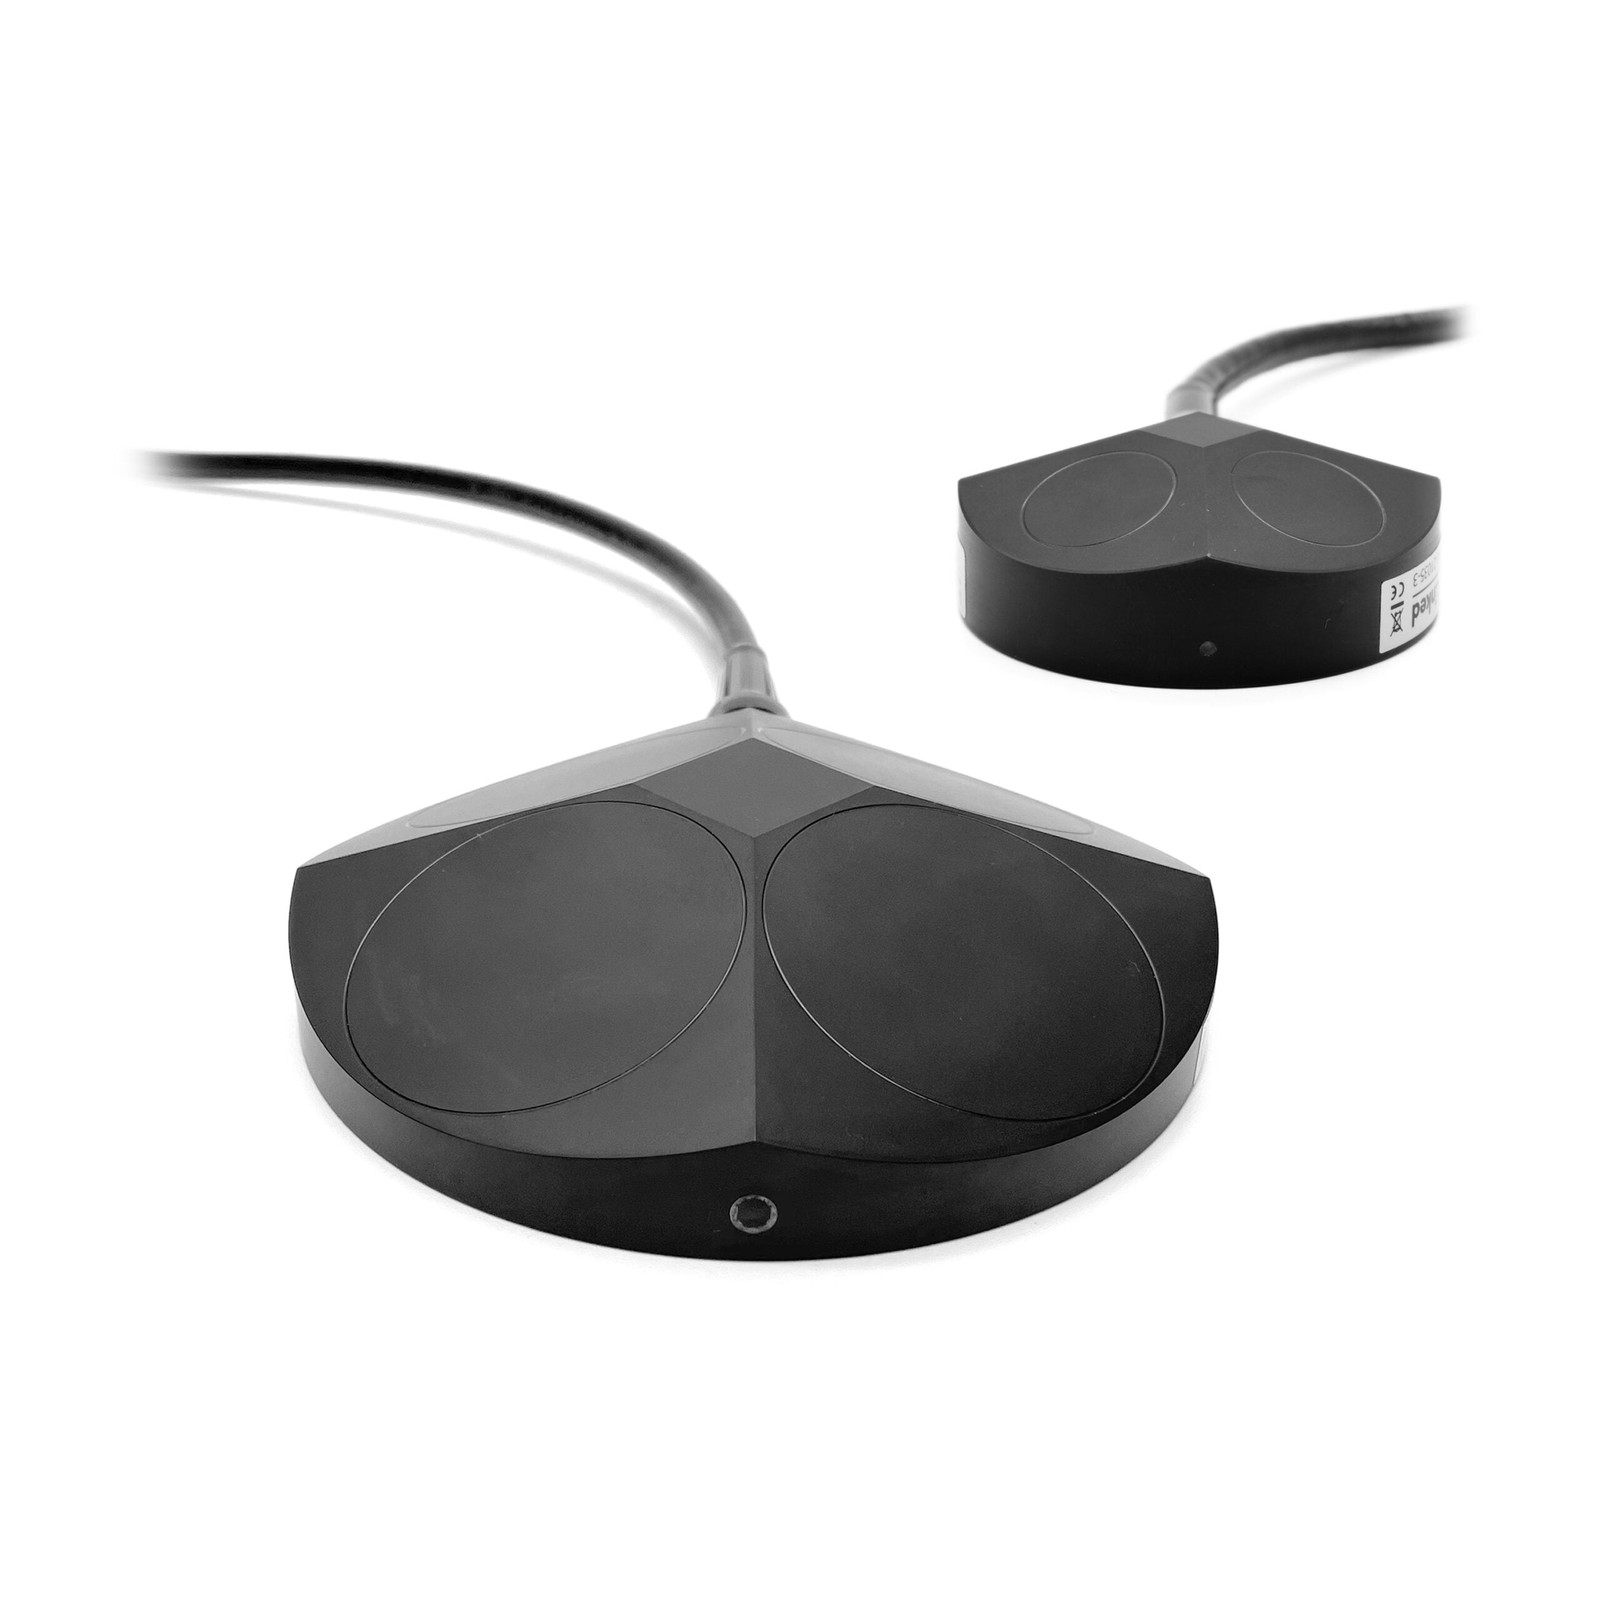
\includegraphics[height=2.3cm, keepaspectratio]{dvl_a50.jpg}\\
        \vspace{0.1em}
        \footnotesize\textbf{Water Linked DVL-A50}\\
        \scriptsize\textit{4 faisceaux Janus 1 MHz, 270 g dans l'eau}
      \end{center}
      \begin{center}
        \begin{tikzpicture}[scale=0.68]
          \draw[thick, fill=OceanMedium!20, rounded corners] (-1.8, 0.7) rectangle (1.8, 1.15);
          \node at (0, 0.92) {\tiny Châssis Sous-Marin};
          \draw[thick, fill=black!80] (-0.7, 0.25) rectangle (0.7, 0.7);
          \node[white] at (0, 0.48) {\tiny DVL};
          \draw[->, line width=1.1pt, OceanCyan] (-0.5, 0.25) -- (-1.4, -0.75);
          \draw[->, line width=1.1pt, OceanCyan] (0.5, 0.25) -- (1.4, -0.75);
          \draw[->, line width=1.1pt, OceanMedium] (-0.2, 0.25) -- (-0.5, -0.75);
          \draw[->, line width=1.1pt, OceanMedium] (0.2, 0.25) -- (0.5, -0.75);
          \draw[thick, fill=brown!30] (-2, -0.75) rectangle (2, -0.98);
          \node at (0, -0.86) {\tiny Fond marin (Bottom-Track)};
        \end{tikzpicture}
      \end{center}
    \end{column}
  \end{columns}
\end{frame}

\begin{frame}{2.12 Positionnement Acoustique Absolu : LBL vs USBL}
  \begin{table}[h]
    \centering
    \scriptsize
    \begin{tabularx}{\textwidth}{p{2.3cm} X X}
      \toprule
      \textbf{Critère} & \textbf{LBL (Long BaseLine)} & \textbf{USBL (Ultra-Short BaseLine)} \\
      \midrule
      \textbf{Principe géométrique} & Réseau de 3 à 4 balises transpondeuses ancrées et calibrées au fond marin autour de la zone & Antenne unique sous la coque / perche surface (matrice d'hydrophones espacés de quelques centimètres) \\
      \textbf{Méthode de calcul} & Triangulation / multilatération par temps de vol (ToF) aller-retour avec chaque balise & Distance par temps de vol (ToF) + \textbf{Gisement \& Site par déphasage} d'onde inter-éléments \\
      \textbf{Précision} & \succw{Centimétrique à décimétrique ($\pm 0.1\,\text{m}$)}, \textbf{indépendante de la profondeur} & Relative à la portée (\alertw{$0.2\%\text{--}1\%$ de la distance oblique}, ex: $\pm 1\,\text{m}$ à $100\,\text{m}$, $\pm 5\,\text{m}$ à $500\,\text{m}$) \\
      \textbf{Logistique \& Déploiement} & \alertw{Très lourde} : mouillage balises, calibration bathymétrique/GNSS par bateau, récupération en fin de manip & \succw{Ultra-légère} : perche sur semi-rigide ou ASV BlueBoat, zéro matériel au fond, suit le navire \\
      \textbf{Zone d'évolution} & Limitée au périmètre balisé ($1\text{--}2\,\text{km}^2$) & Mobile, suit le bateau support sans limite de zone \\
      \textbf{Sensibilité attitude} & Insensible aux mouvements de surface & \alertw{Critique} : nécessite une centrale d'attitude (MRU/IMU) en surface pour compenser roulis/tangage \\
      \bottomrule
    \end{tabularx}
  \end{table}
\end{frame}

\begin{frame}{2.12b Matériel Acoustique Réel : Balises LBL \& Transceivers USBL}
  \begin{columns}[c]
    \begin{column}{0.48\textwidth}
      \begin{center}
        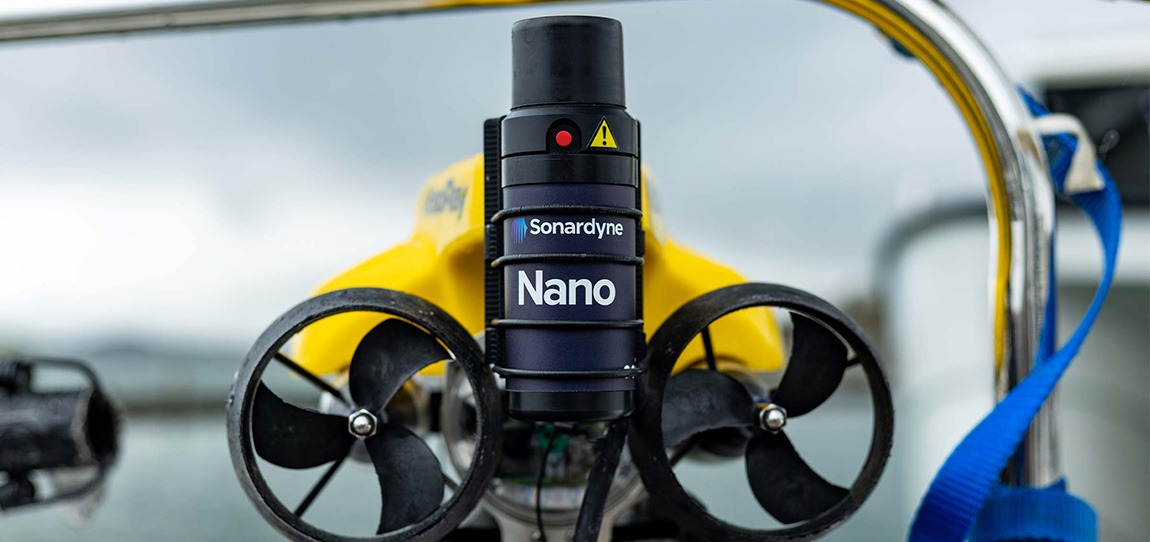
\includegraphics[height=1.8cm, keepaspectratio]{lbl_nano_transponder.jpg}
        \hspace{0.2cm}
        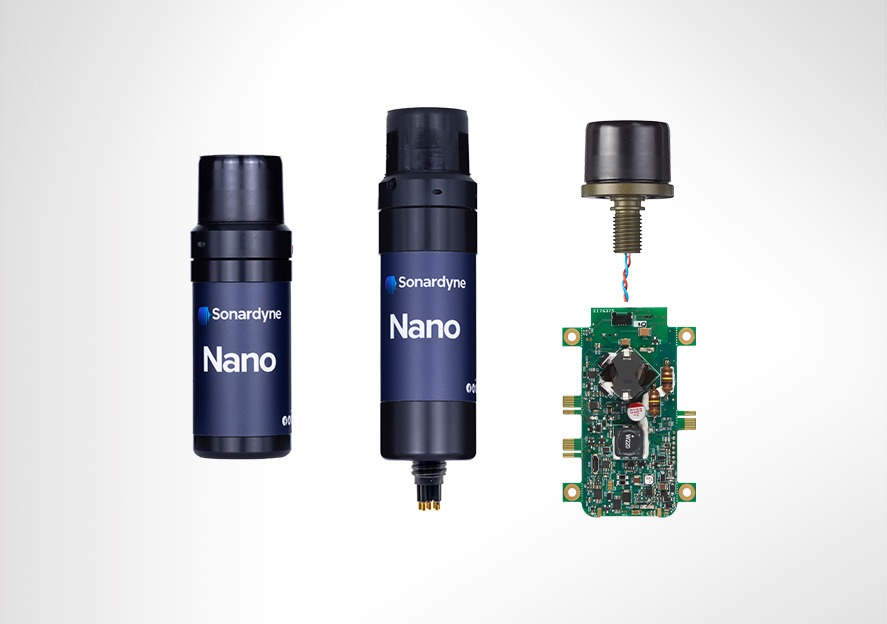
\includegraphics[height=1.8cm, keepaspectratio]{lbl_nano_beacon.jpg}\\
        \vspace{0.2em}
        \tech{Balise Transpondeuse LBL \& Ancrage}\\
        \tiny\textit{Réseau de fond fixe $\cdot$ Triangulation ToF centimétrique}
      \end{center}
      \scriptsize
      \begin{block}{Fonctionnement LBL Réel}
        Balise autonome sur batterie immergée au fond. Répond par un ping codé lorsqu'elle est interrogée par le robot.
      \end{block}
    \end{column}

    \begin{column}{0.48\textwidth}
      \begin{center}
        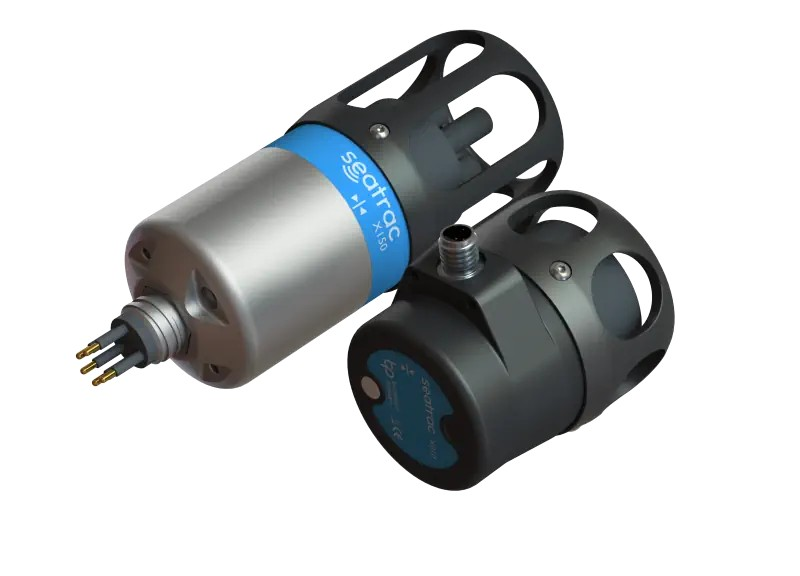
\includegraphics[height=1.8cm, keepaspectratio]{seatrac_usbl_photo.jpg}
        \hspace{0.2cm}
        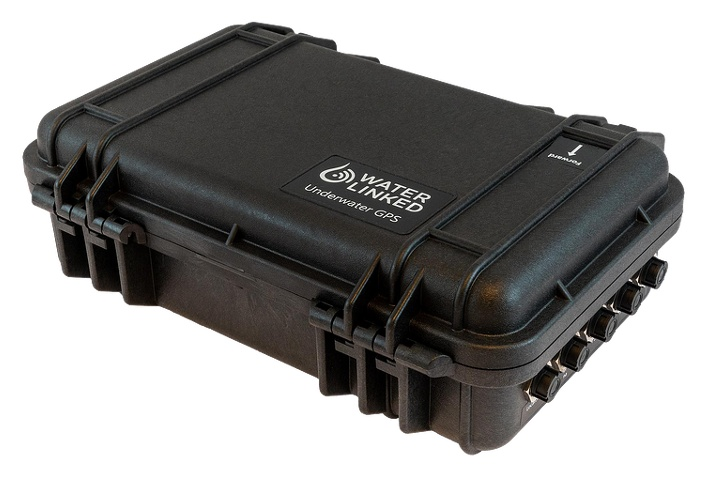
\includegraphics[height=1.8cm, keepaspectratio]{waterlinked_ugps.jpg}\\
        \vspace{0.2em}
        \succw{Antenne USBL Surface \& Transpondeur ROV}\\
        \tiny\textit{Systèmes SeaTrac X150 / Water Linked UGPS $\cdot$ Perche de surface}
      \end{center}
      \scriptsize
      \begin{block}{Fonctionnement USBL Réel}
        Matrice multi-hydrophones de surface mesurant les micro-déphasages d'angle d'arrivée ($\theta, \phi$) + temps de vol.
      \end{block}
    \end{column}
  \end{columns}
\end{frame}

\begin{frame}{2.13 Démocratisation USBL \& Télémétrie Acoustique ($\approx 5\,000$ €)}
  \begin{columns}[T, onlytextwidth]
    \begin{column}{0.44\textwidth}
      \begin{block}{\tech{1. Démocratisation des USBL}}
        \scriptsize
        \begin{itemize}\setlength{\itemsep}{2pt}\setlength{\parskip}{0pt}
          \item \textbf{Rupture de coût} : autrefois réservé à l'offshore ($>50\text{--}100\,\text{k€}$), désormais accessible aux labos (\succw{$\mathbf{\approx 5\text{--}8\,\text{k€}}$}, ex. \tech{Water Linked UGPS}, \tech{SeaTrac}).
          \item \textbf{Déploiement léger} : perche sur semi-rigide ou drone de surface ASV (\tech{BlueBoat}).
        \end{itemize}
      \end{block}

      \vspace{-0.15em}
      \begin{block}{\succw{2. Double Rôle : Position \& Télémesure}}
        \scriptsize
        \begin{itemize}\setlength{\itemsep}{2pt}\setlength{\parskip}{0pt}
          \item \textbf{Modem acoustique intégré} : données numériques modulées sur les pings (chirp / FSK, \textbf{quelques kbps}).
          \item \textbf{Voie montante} ($\uparrow$) : télémétrie vitale (profondeur Bar30, tension batterie, alarmes SOS / fuite).
          \item \textbf{Voie descendante} ($\downarrow$) : recalage fix GNSS absolu, ordres et waypoints de navigation.
        \end{itemize}
      \end{block}
    \end{column}

    \begin{column}{0.54\textwidth}
      \centering
      \begin{tikzpicture}[scale=0.92, every node/.style={transform shape}]
        % 1. Environnement : Ciel, Eau et Fond marin
        \fill[blue!4!white] (-4.0, 1.45) rectangle (4.0, 3.10);
        \fill[OceanCyan!8] (-4.0, -2.40) rectangle (4.0, 1.45);
        \fill[brown!22] (-4.0, -2.85) rectangle (4.0, -2.40);
        \draw[OceanMedium!40, line width=0.8pt, rounded corners=4pt] (-4.0, -2.85) rectangle (4.0, 3.10);

        % Ligne de surface (eau)
        \draw[OceanCyan, dashed, line width=0.9pt] (-4.0, 1.45) -- (4.0, 1.45);
        \node[OceanCyan!85!black, font=\fontsize{5}{6}\selectfont\bfseries, anchor=north west] at (-3.85, 1.35) {Surface (Eau de mer)};

        % Ligne de fond marin
        \draw[brown!60!black, thick] (-4.0, -2.40) -- (4.0, -2.40);
        \node[brown!80!black, font=\fontsize{5.5}{6.5}\selectfont\bfseries, anchor=west] at (-3.85, -2.62) {Fond marin (Bathymétrie)};
        \node[DarkSlate, font=\fontsize{4.8}{5.8}\selectfont, anchor=east] at (3.80, -2.62) {Portée : 50 à 500\,m};

        % 2. Cartouche 1 : Géoréférencement USBL (Dans le ciel / surface en haut à gauche)
        \node[anchor=north west, fill=white, fill opacity=0.96, text opacity=1, draw=OceanCyan, line width=0.8pt, rounded corners=3pt, inner sep=3pt, drop shadow={opacity=0.08}] at (-3.9, 3.02) {%
          \begin{minipage}{4.0cm}
            \textcolor{OceanDeep}{\textbf{\scriptsize 1. Géoréférencement USBL}}\\[1pt]
            \centering
            {\scriptsize\succw{$\vec{X}_{\text{AUV}} = \vec{X}_{\text{GNSS}} + \mathbf{R}_{\text{bateau}} \cdot \vec{P}_{\text{USBL}}$}}\\[2pt]
            \raggedright\fontsize{5}{6}\selectfont
            $\bullet$ \textbf{Distance $D$} : temps de vol aller-retour ($\Delta t$)\\
            $\bullet$ \textbf{Direction $(\theta, \psi)$} : déphasage hydrophones\\
            $\implies$ Fix GNSS absolu injecté dans l'AUV
          \end{minipage}
        };

        % 3. Bateau support / ASV de surface (BlueBoat)
        \draw[thick, fill=white, draw=OceanDeep, rounded corners=2pt] (0.8, 1.4) -- (1.2, 2.15) -- (3.8, 2.15) -- (3.4, 1.4) -- cycle;
        \node[font=\scriptsize\bfseries, text=OceanDeep] at (2.4, 1.78) {ASV Surface};

        % Mât et antenne GNSS RTK
        \draw[line width=1.4pt, DarkSlate] (3.2, 2.15) -- (3.2, 2.75);
        \fill[OceanDeep] (3.2, 2.75) circle (2.8pt);
        \draw[OceanDeep, line width=0.6pt] (3.06, 2.82) arc[start angle=150, end angle=30, radius=0.16];
        \draw[OceanDeep, line width=0.6pt] (2.96, 2.89) arc[start angle=150, end angle=30, radius=0.27];
        \node[anchor=south east, font=\tiny\bfseries, text=OceanDeep] at (3.05, 2.5) {GNSS};
        \node[anchor=south east, font=\fontsize{5}{6}\selectfont, text=OceanMedium] at (3.05, 2.22) {Fix $\vec{X}_{\text{surf}}$};

        % Perche rigide et Antenne USBL immergée
        \draw[line width=2.6pt, DarkSlate] (1.35, 1.4) -- (1.35, 0.42);
        \draw[line width=0.8pt, fill=DarkSlate, rounded corners=1pt] (1.10, 0.30) rectangle (1.60, 0.44);
        \fill[OceanCoral] (1.35, 0.26) circle (4.2pt);
        \fill[white] (1.23, 0.26) circle (1pt);
        \fill[white] (1.47, 0.26) circle (1pt);
        \node[anchor=west, font=\tiny\bfseries, text=OceanCoral] at (1.75, 0.40) {Tête USBL};
        \node[anchor=west, font=\fontsize{4.8}{5.8}\selectfont, text=DarkSlate] at (1.75, 0.20) {(4 hydrophones)};

        % 4. Véhicule sous-marin (AUV / BlueROV2)
        \draw[line width=1.1pt, fill=OceanMedium!15, draw=OceanDeep, rounded corners=4pt] (-3.5, -2.25) rectangle (-1.5, -1.65);
        \node[font=\scriptsize\bfseries, text=OceanDeep] at (-2.5, -1.95) {AUV};
        % Propulseurs
        \fill[DarkSlate] (-3.68, -2.18) rectangle (-3.5, -2.04);
        \fill[DarkSlate] (-3.68, -1.86) rectangle (-3.5, -1.72);
        % Capteur Bar30
        \fill[OceanCyan] (-1.5, -1.95) circle (2.2pt);
        \node[anchor=west, font=\fontsize{4.8}{5.8}\selectfont, text=OceanMedium] at (-1.45, -1.95) {Bar30 ($z$)};
        % Transpondeur acoustique
        \draw[line width=1pt, fill=DarkSlate] (-2.25, -1.65) rectangle (-1.95, -1.40);
        \fill[OceanCoral] (-2.1, -1.33) circle (3.5pt);
        \node[anchor=south east, font=\tiny\bfseries, text=OceanCoral] at (-2.2, -1.35) {Transpondeur};

        % 5. Fronts d'ondes acoustiques stylisés
        \draw[OceanCyan!30, line width=1pt] (0.95, 0.05) arc[start angle=195, end angle=235, radius=0.6];
        \draw[OceanCyan!30, line width=1.1pt] (0.45, -0.18) arc[start angle=195, end angle=235, radius=1.2];
        \draw[OceanCyan!30, line width=1.2pt] (-0.05, -0.42) arc[start angle=195, end angle=235, radius=1.8];

        % 6. Faisceaux acoustiques (Pings & Modem)
        % Faisceau USBL
        \draw[{Latex[length=2.2mm]}-{Latex[length=2.2mm]}, line width=2.0pt, OceanCyan] (1.10, 0.12) -- (-1.80, -1.22);
        \node[pos=0.44, sloped, above=3pt, fill=white, fill opacity=0.94, text opacity=1, draw=OceanCyan!70, rounded corners=2pt, inner sep=1.6pt, font=\fontsize{5.2}{6.2}\selectfont\bfseries, text=OceanMedium] {1. Pings USBL (ToF + Déphasage)};

        % Faisceau Modem
        \draw[{Latex[length=1.8mm]}-{Latex[length=1.8mm]}, line width=1.6pt, OceanGreen, dashed] (1.25, -0.06) -- (-1.65, -1.38);
        \node[pos=0.44, sloped, below=3pt, fill=white, fill opacity=0.94, text opacity=1, draw=OceanGreen!70, rounded corners=2pt, inner sep=1.6pt, font=\fontsize{5.2}{6.2}\selectfont\bfseries, text=OceanGreen!80!black] {2. Modem Acoustique ($\uparrow\downarrow$ Données \& Ordres)};

        % 7. Cartouche 2 : Modem Acoustique (Coin inférieur droit)
        \node[anchor=north west, fill=white, fill opacity=0.96, text opacity=1, draw=OceanGreen, line width=0.8pt, rounded corners=3pt, inner sep=3pt, drop shadow={opacity=0.08}] at (0.5, -0.60) {%
          \begin{minipage}{3.3cm}
            \textcolor{OceanDeep}{\textbf{\scriptsize 2. Liaison Acoustique Sans Fil}}\\[1pt]
            \fontsize{5}{6}\selectfont
            \succw{$\blacktriangledown$} \textbf{Descendant (Surface $\rightarrow$ Robot)} :\\
            \quad $\cdot$ Recalage Kalman (fix GNSS absolu)\\
            \quad $\cdot$ Consignes, waypoints, arrêt SOS\\[1.5pt]
            \alertw{$\blacktriangle$} \textbf{Montant (Robot $\rightarrow$ Surface)} :\\
            \quad $\cdot$ Profondeur Bar30 ($z$), tension Li-Ion,\\
            \quad $\cdot$ Alarmes SOS \& détection de fuite
          \end{minipage}
        };
      \end{tikzpicture}
    \end{column}
  \end{columns}
\end{frame}

\begin{frame}{2.14 Propagation Acoustique \& Pièges de Terrain}
  \begin{columns}[T]
    \begin{column}{0.49\textwidth}
      \begin{block}{\tech{1. Célérité $c(z)$ \& Réfraction (Loi de Snell)}}
        \scriptsize
        \begin{itemize}
          \item La célérité $c(S,T,P) \approx 1450\text{--}1540\,\text{m/s}$ varie selon la thermocline et la pycnocline.
          \item Réfraction : les rayons acoustiques se courbent systématiquement vers les couches où le son est plus lent ($\frac{\cos\theta}{c} = \text{cte}$).
          \item \alertw{Création de zones d'ombre} (zones de silence où aucun ping ne passe) et erreurs de distance si $c(z)$ n'est pas mesuré par sonde CTD/SVP.
        \end{itemize}
      \end{block}

      \begin{block}{\alertw{2. Multi-trajets}}
        \scriptsize
        \begin{itemize}
          \item Réflexions parasites sur l'interface air-eau et sur le fond marin.
          \item Arrivée d'échos multiples déphasés qui brouillent le signal direct : critique par \textbf{petits fonds ($<15\,\text{m}$)}, bassins et zones portuaires.
        \end{itemize}
      \end{block}
    \end{column}

    \begin{column}{0.49\textwidth}
      \begin{block}{\alertw{3. Masquages Géométriques}}
        \scriptsize
        \begin{itemize}
          \item \textbf{Relief sous-marin} : dômes rocheux, canyons, surplombs, épaves et piliers de quai qui coupent la ligne de visée acoustique (*Line-of-Sight*).
          \item \textbf{Vecteur porteur} : masquage par la coque du bateau ou l'ombilical.
        \end{itemize}
      \end{block}

      \begin{block}{\succw{4. Bruits Ambiants \& Atténuation}}
        \scriptsize
        \begin{itemize}
          \item \textbf{Aération de surface} : bulles d'air sous la coque formant un écran opaque aux ondes sonores.
          \item \textbf{Cavitation \& moteurs} : bruit des hélices à forte poussée couvrant les signaux de faible amplitude.
          \item \textbf{Atténuation avec la fréquence} : haute fréquence ($>100\,\text{kHz}$) = portée courte ($<100\,\text{m}$).
        \end{itemize}
      \end{block}
    \end{column}
  \end{columns}
\end{frame}
